\documentclass[xcolor={dvipsnames}]{beamer}
\usepackage{amsmath}
\usepackage{amsfonts}
\usepackage{mathtools}
\usepackage{xparse}

\usepackage[T1]{fontenc} 	% Code blocks!
\usepackage{listings} 		% Code blocks!
\usepackage{textcomp} 		% Code blocks.
\usepackage{sourcecodepro}  % Better font?
\usepackage{upquote}
\usepackage{microtype}      % Suppress ligatures.

% No ligatures for ttfamily.
\DisableLigatures{encoding = T1, family = tt*}


\usepackage{graphicx}
\graphicspath{{./img/}{./img/content/}}

% CTF GOOOOOOOOOO!
\usetheme{Firebird}

\usepackage{hyperref}
\definecolor{links}{HTML}{2A1B81}
\hypersetup{colorlinks,linkcolor=,urlcolor=links}
\usepackage{url}

% External hyperlink, different from the colourless internal links used in Beamer navigation.
% May require [fragile] in slides.
\NewDocumentCommand\exref{v m}{\href{#1}{\color{links}{\underline{#2}}}}

% Tikz stuff.
\usepackage{tikzit}         % https://tikzit.github.io/
\input{figures/styles.tikzstyles}
\input{figures/styles.tikzdefs}
\usepackage{tikzpagenodes}

\usepackage[absolute,overlay]{textpos}
\setlength{\TPHorizModule}{10mm}
\setlength{\TPVertModule}{10mm}

% Convenience command for drawing a grid.
\newcommand\ShowGrid{%
    \tikz[
        remember picture,
        overlay,
        yscale=-1,
        xstep=\TPHorizModule,ystep=\TPVertModule]
    \draw (current page.north west) grid (current page.south east);}

\newenvironment{overlaytextblock}{\TPoptions{absolute=false,overlay=false}}{\TPoptions{absolute=true,overlay=true}}

\usepackage{rotating}   % https://en.wikibooks.org/wiki/LaTeX/Rotations

\usepackage{setspace}

% Convenience wrapper for bracketing. \delim* for auto-sizing, \delim[\bigg] for manual sizing.
\DeclarePairedDelimiter\ceil{\lceil}{\rceil}
\DeclarePairedDelimiter\floor{\lfloor}{\rfloor}
\DeclarePairedDelimiter\abs{\lvert}{\rvert}
\DeclarePairedDelimiter\parens{(}{)}
\DeclarePairedDelimiter\angles{\langle}{\rangle}

%%%% Useful Macros %%%
\renewcommand{\o}{\varnothing} % Empty set.
\newcommand{\N}{\mathbb{N}} % Natural numbers.
\newcommand{\Z}{\mathbb{Z}} % Integers.
\newcommand{\Q}{\mathbb{Q}} % Rational numbers.
\newcommand{\R}{\mathbb{R}} % Real numbers.
\newcommand{\C}{\mathbb{C}} % Complex numbers.
\newcommand{\powerset}{\mathcal{P}} % Power set.
\newcommand{\insum}{\textstyle\sum} % Inline summation.
\newcommand{\st}{\text{ such that }} % Inline text.
\newcommand{\order}{\text{order}} % Inline summation.
\newcommand{\lcm}{\text{lcm}} % Inline summation.
\newcommand{\Ker}[1]{\text{Ker}\parens*{#1}} % Kernel.

\renewcommand{\epsilon}{\varepsilon}
\renewcommand{\b}[1]{\!\left(#1\right)}

\newcommand{\xor}{\oplus}
\newcommand{\cnot}{\centernot}

\newcommand{\code}[1]{\texttt{#1}}
\newcommand{\codec}[1]{{\color{orange!90!black}\texttt{#1}}}
\newcommand{\codel}[1]{\lstinline{#1}}
% \NewDocumentCommand{\codel}{O{} m}{\lstinline[#1]{#2}}

\newcommand{\arr}{\rightarrow\,}

% Slide settings.
\beamertemplatenavigationsymbolsempty % No nav bar. >:)
\NewDocumentCommand{\slideref}{mo}{\hyperlink{#1}{\IfNoValueTF {#2} {Slide~\ref*{#1}} {Slide~\ref*{#1}~#2}}}

% Slide footnote size.
\newcommand{\slidefnsize}{\tiny}

\NewDocumentCommand{\absfootnote}{m}{%
    \begin{textblock}{10}(1,9.35)%
        \slidefnsize #1%
    \end{textblock}%
}

\NewDocumentCommand{\absfootnoteb}{m}{%
    \begin{textblock}{10}(1,9.05)%
        \slidefnsize #1%
    \end{textblock}%
}

% Requires [fragile] on frames.
\NewDocumentCommand{\morefootnote}{O{More} v}{%
    \begin{textblock}{10}(1,9.35)%
        \slidefnsize {#1}: {\url{#2}}.%
    \end{textblock}%
}

% Absolute-positioned graphic.
\NewDocumentCommand{\absgraphic} {m O{0cm} O{0cm}} {
    \begin{tikzpicture}[remember picture,overlay,shift={(current page.north west)}]
        \node[anchor=north west,xshift=#2,yshift=#3]{#1};
    \end{tikzpicture}}

% Line spacing.
\setstretch{1.15}

% Code format.

%% Usage:
% \begin{lstlisting}[style=plain(, options=...)]
% # Code goes here.
% \end{lstlisting}

\lstset{
    basicstyle = \ttfamily\color{black},
    keywordstyle = \color{blue!80},
    stringstyle = \color{Mahogany},
    % backgroundcolor = \color{WhiteSmoke},
    breaklines = true,
    % escapeinside = {(*}{*)},                   % For adding LaTeX in code. (* 1+1 *)
    extendedchars = true,
    frame = none,
    % identifierstyle = \color{blue},
    keepspaces = true,
    language = Python,                   		% Change the programming language here!
    mathescape = true,
    morekeywords = {*, None},
    numbers = none, 							% Line-numbers (possible values: none, left, right).
    numbersep = 10pt,                   		% Distance between line-numbers and code
    numberstyle=\color{darkgray}, 		        % Style used for line-numbers.
    rulecolor = \color{black},
    showstringspaces = false,
    tabsize = 4,
    upquote = true,
}

\lstdefinestyle{plainc}{
    tabsize = 4,
    language = C,
    basicstyle = \footnotesize\ttfamily\color{black},
    commentstyle = \color{teal},
    keywordstyle = \color{blue!80},
    stringstyle = \color{Mahogany},
}

\lstdefinestyle{plainpy}{
    basicstyle = \footnotesize\ttfamily\color{black},
    commentstyle = \color{teal},
    keywordstyle = \color{blue!80},
    stringstyle = \color{Mahogany},
    moredelim = **[is][\only<+>{\color{black}}]{@}{@},
}

\lstdefinestyle{focuspy}{
    % Lighter by default.
    basicstyle = \footnotesize\ttfamily\color{black!40},
    commentstyle = \itshape\color{teal!40},
    keywordstyle = \color{blue!40},
    stringstyle = \color{Mahogany!50},
    % morekeywords = {*},
    moredelim = **[is][\only<+>{\color{black}\lstset{style=plainpy}}]{@}{@},
}

\lstdefinestyle{plain2}{
    basicstyle = \footnotesize\ttfamily\color{black},
    commentstyle = \ttfamily\color{black},
    stringstyle = \color{Mahogany},
    morekeywords = [1]{int, bool, bytes, BV, SimState, None},
    keywordstyle = [1]\color{blue!80},
    morekeywords = [2]{eval},
    keywordstyle = [2]\color{black},
    moredelim = [is][\color{black}\lstset{keywordstyle=\color{black}}]{<<}{>>},
    moredelim = **[is][\only<+>{\color{black}}]{@}{@},
}
\lstdefinestyle{focus2}{
    basicstyle = \footnotesize\ttfamily\color{black!40},
    commentstyle = \ttfamily\color{black!40},
    stringstyle = \color{Mahogany!50},
    morekeywords = [1]{int, bool, bytes, BV, SimState, None},
    keywordstyle = [1]\color{blue!40},
    morekeywords = [2]{eval},
    keywordstyle = [2]\color{black!40},
    moredelim = [is][\color{black}\lstset{keywordstyle=\color{black}}]{<<}{>>},
    moredelim = **[is][\only<+>{\color{black}\lstset{style=plain2}}]{@}{@},
}

% hybrid2: if in handout mode, use plainpy. If in beamer mode, use focuspy.
\mode<handout>{\lstdefinestyle{hybridpy}{style=plainpy}}
\mode<beamer>{\lstdefinestyle{hybridpy}{style=focuspy}}

\mode<handout>{\lstdefinestyle{hybrid2}{style=plain2}}
\mode<beamer>{\lstdefinestyle{hybrid2}{style=focus2}}



\title[Advanced angr]{SOMP1010: angr Management}
\subtitle{Crack binaries with righteous indignation!}
\date{May 6, 2022}
\author{TrebledJ}


\begin{document}
\TitlePage

\subsection{Preamble}
\begin{frame}{Code of Ethics}
    \begin{spacing}{1}
        \begin{itemize}
            \item {\footnotesize The exercises for the course should be attempted ONLY INSIDE THE SECLUDED LAB ENVIRONMENT documented or provided. Please note that most of the attacks described in the slides would be ILLEGAL if attempted on machines that you do not have explicit permission to test and attack. The university, course lecturer, lab instructors, teaching assistants and the Firebird CTF team assume no responsibility for any actions performed outside the secluded lab.}

            \item {\footnotesize Do not intentionally disrupt other students who are working on the challenges or disclose private information you found on the challenge server (e.g. IP address of other students).}

            \pause
            \item {\footnotesize When solving CTF challenges or hunting angr documentation for some obscure class, it is imperative that you remain calm. Do not destroy the challenge server or make stupid decisions out of frustration or angr!}
        \end{itemize}
    \end{spacing}
\end{frame}

\subsection{Preamble}
\begin{frame}[fragile]{Today's Talk}
    \begin{itemize}
        \item<1-> Reverse!
        \item<2-> Less focus on angr's API
        \item<2-> More focus on the big picture
        \item<2-> More memes
        \item<3-> Unrelated to the \exref{https://github.com/angr/angr-management}{GUI tool}
    \end{itemize}
    \absgraphic{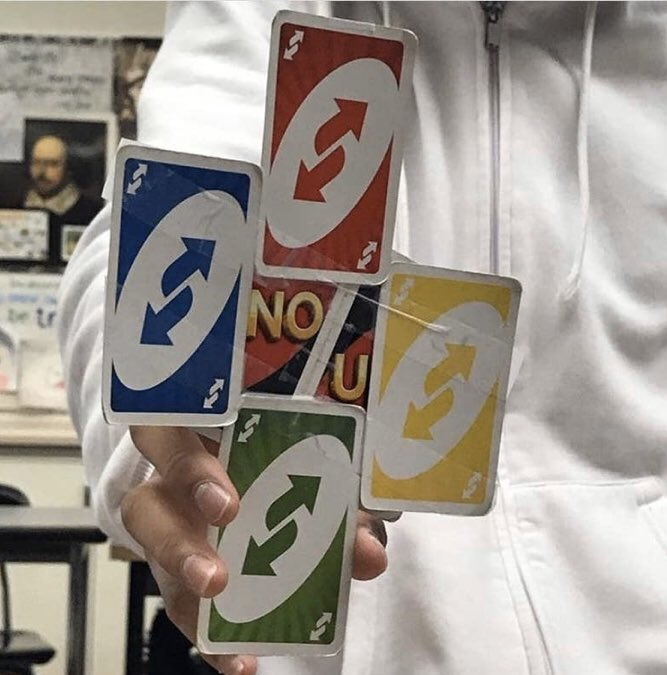
\includegraphics[width=4cm]{reverse-1}}[8cm][-1.8cm]
    \absgraphic{
\includegraphics[width=4cm]{reverse-2}}[8cm][-6.2cm]
\end{frame}

\subsection{Preamble}
\begin{frame}{How to Manage Your angr}
    \tableofcontents[hideallsubsections]
\end{frame}


\section{Introduction}
\frame{\sectionpage}
\begin{frame}{What is this angr?}
    Highly modularised and customisable framework for...
    \begin{itemize}
        \item Symbolic execution
        \item Binary analysis (control flow, value set, dependencies)
        \item Reversing binaries with righteous indignation
    \end{itemize}
    \-\\
    \begin{uncoverenv}<2->
        Repo: \url{https://github.com/angr/angr} \\
        Docs (Book-like): \url{https://docs.angr.io/} \\
        API: \url{https://api.angr.io/}
    \end{uncoverenv}

    \absfootnote{See \slideref{tips}[for angr setup tips!]}
    \absgraphic{
\includegraphics[width=2.5cm]{inside-out-anger}}[9cm][-7cm]
\end{frame}

\subsection{Motivation}
\begin{frame}{Motivation}
    % HKCERT21 step-by-step.
    \vskip5pt
    \centering
    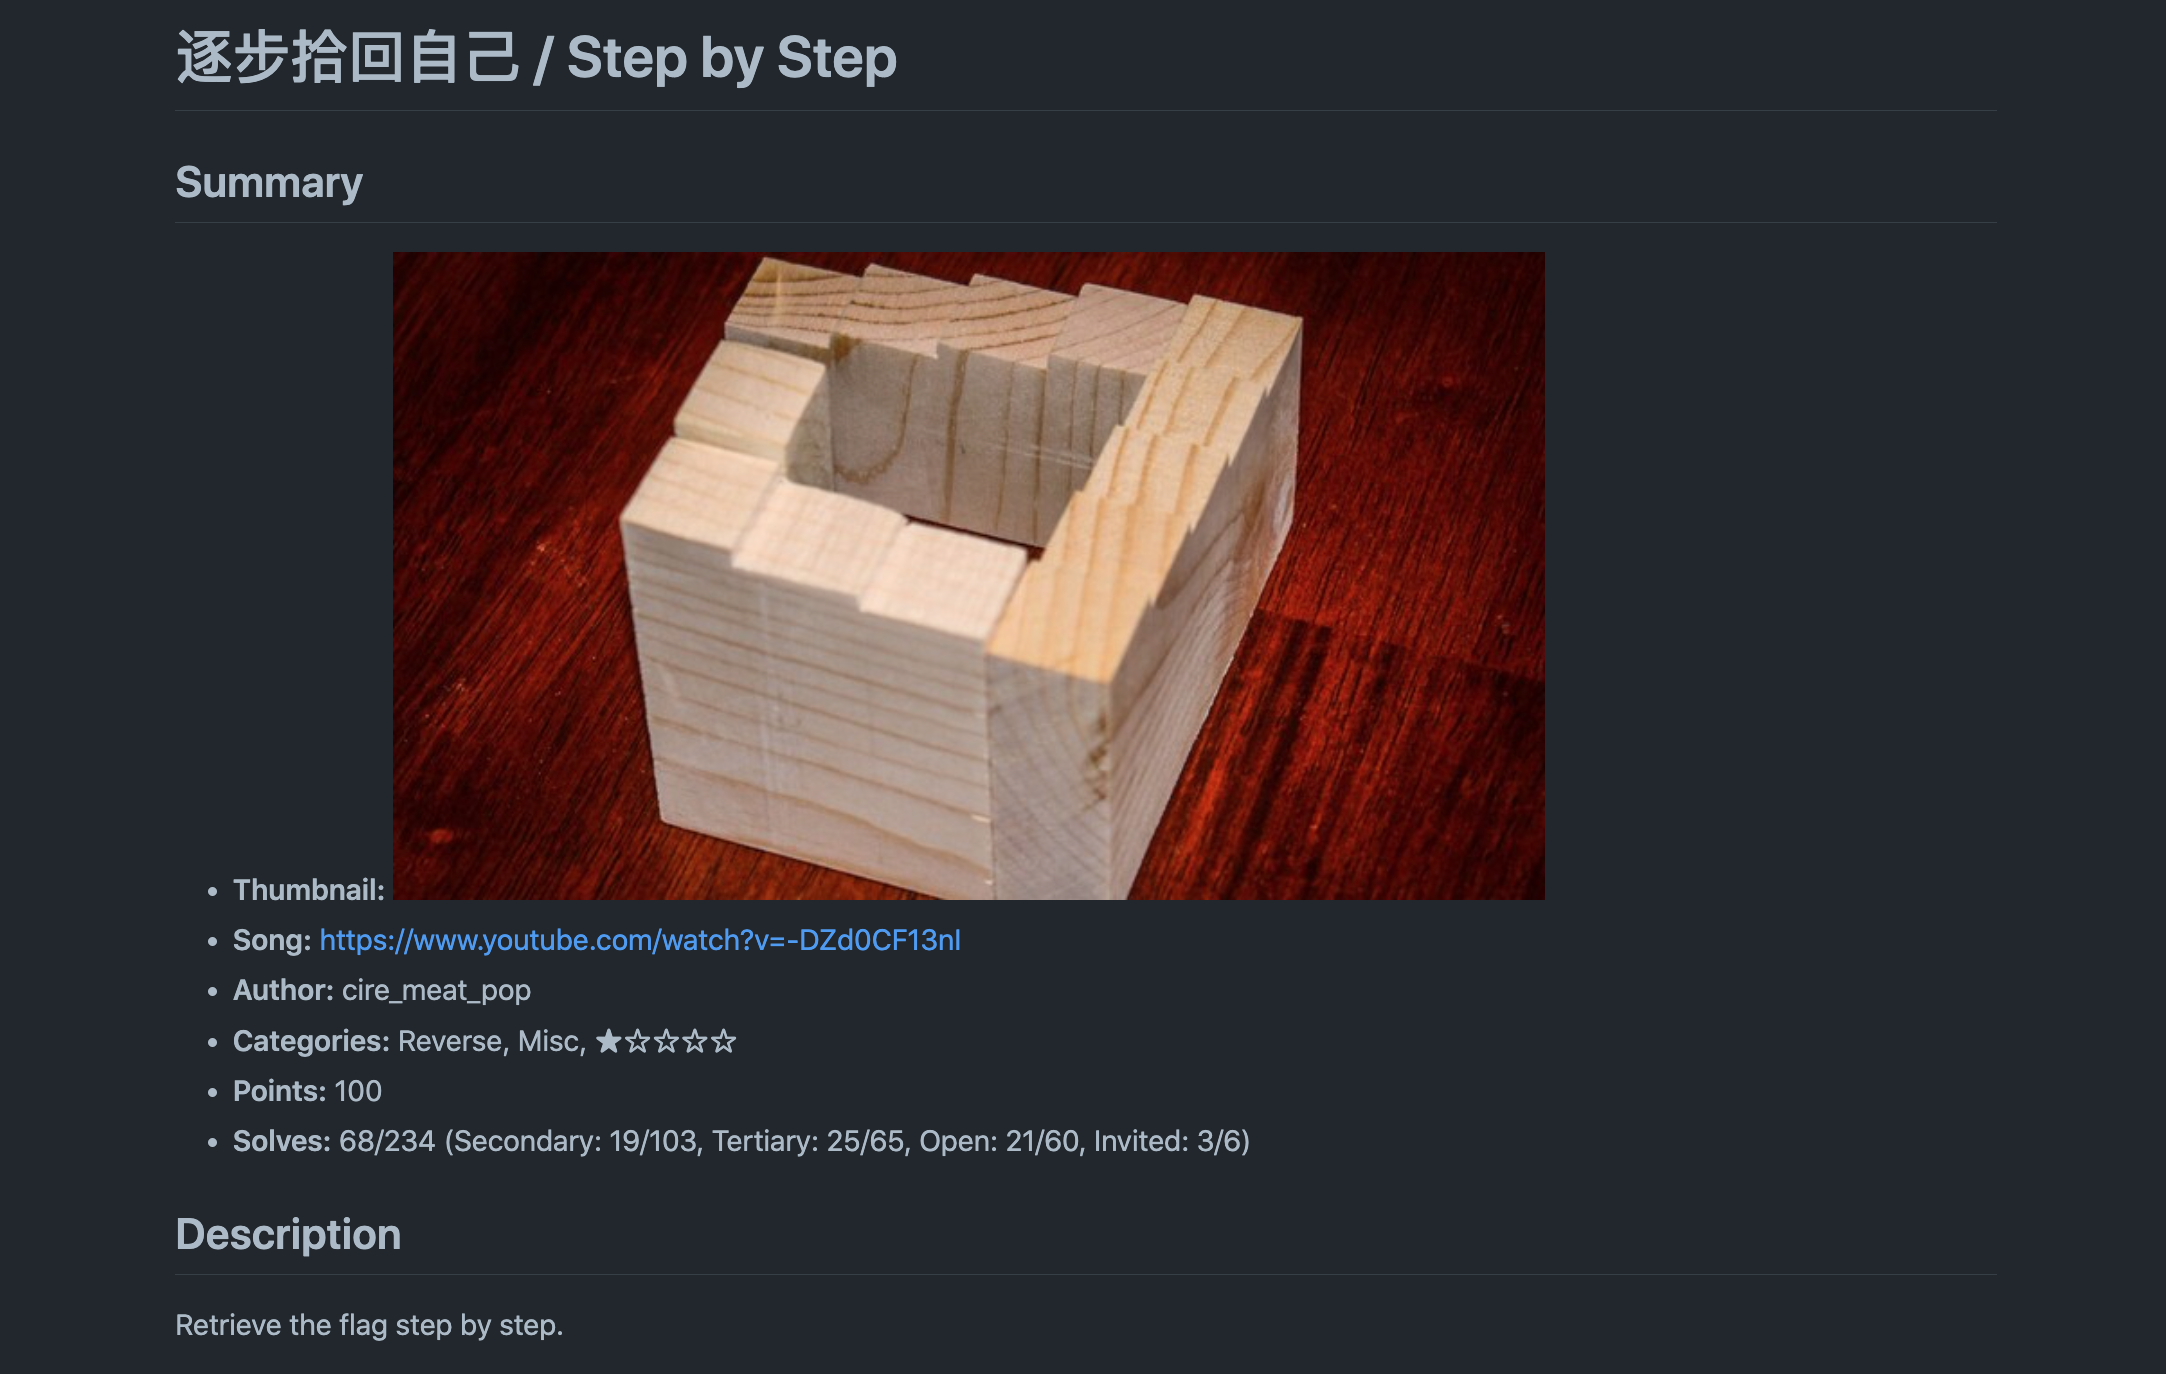
\includegraphics[width=0.95\textwidth]{chal-step-by-step}
    \absgraphic{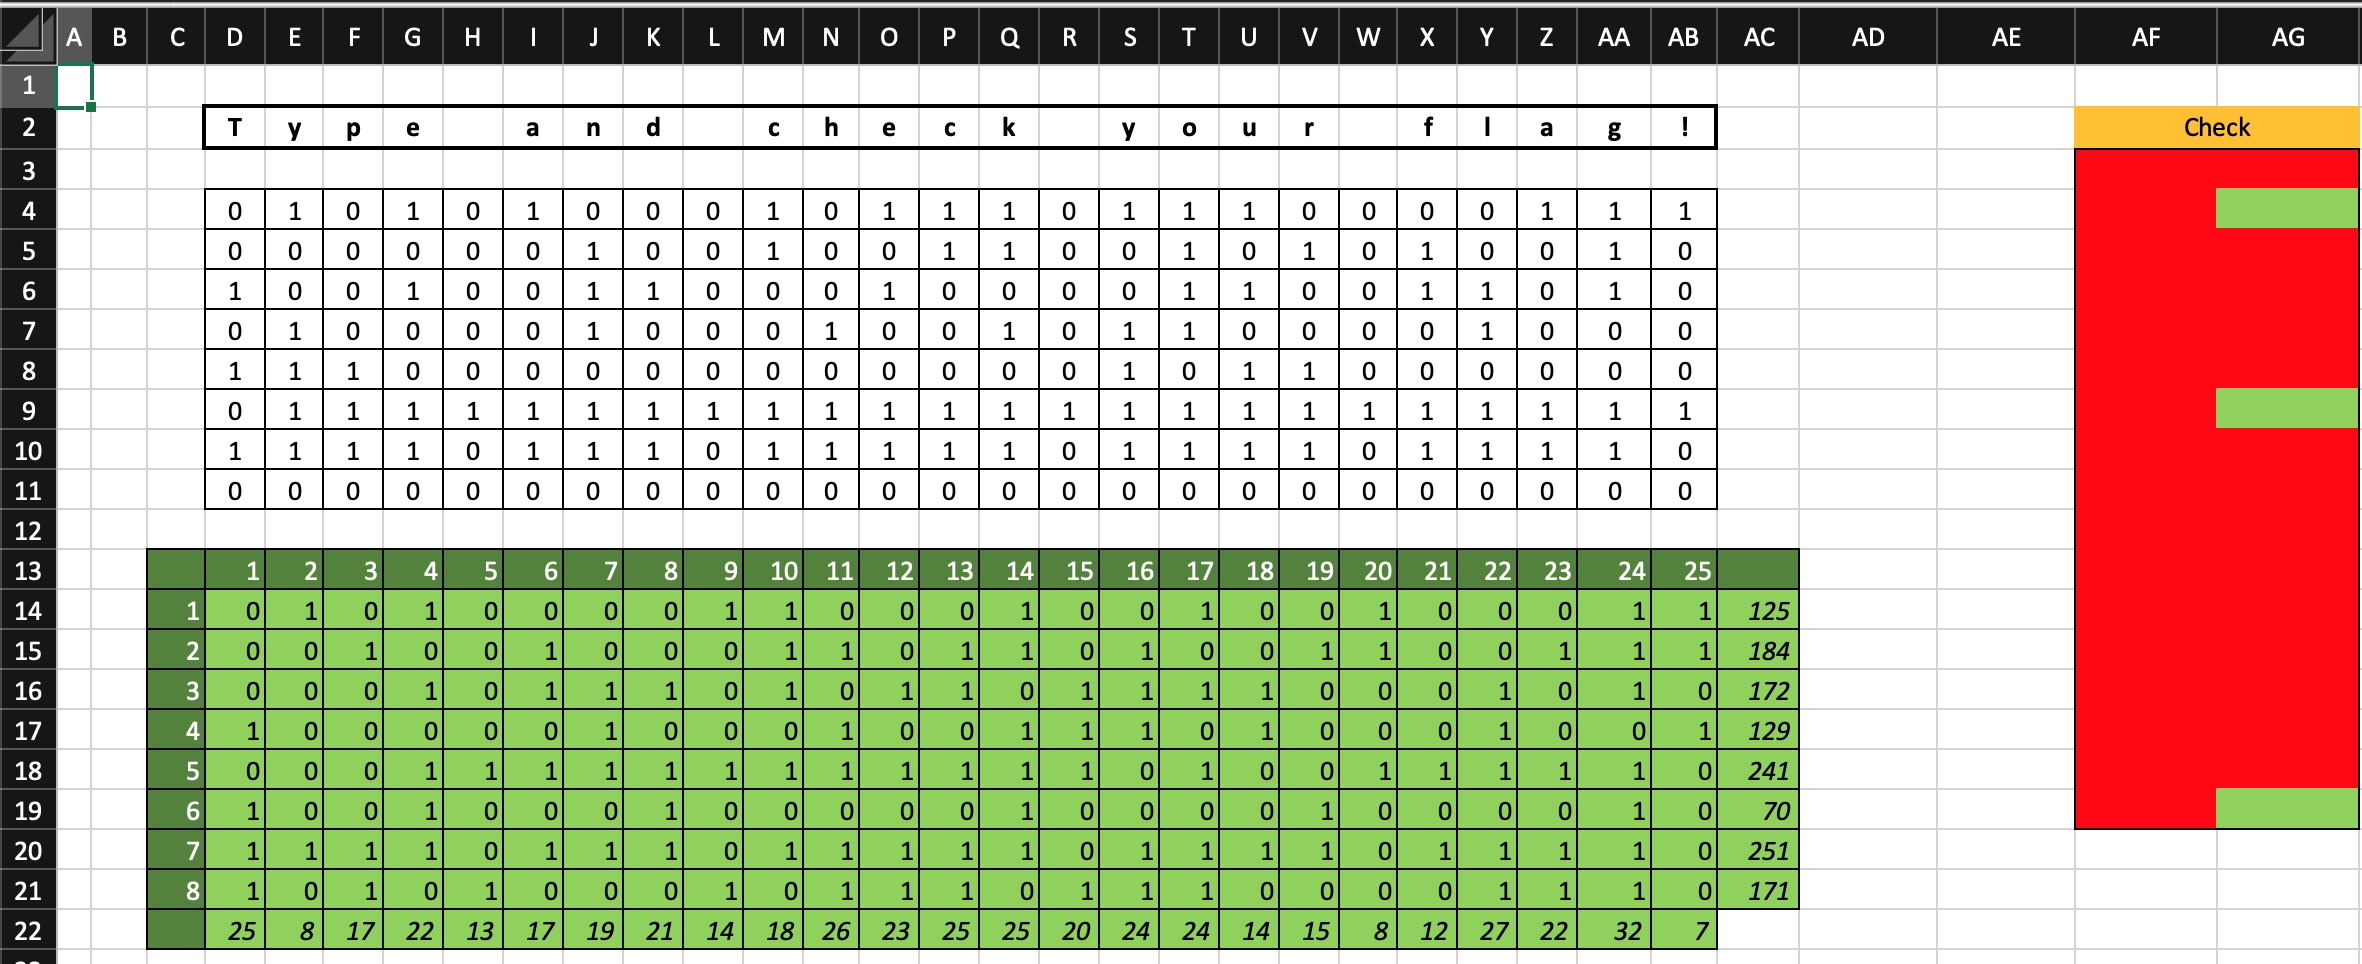
\includegraphics[width=6cm]{step-by-step-excel}}[6cm][-7cm]
\end{frame}
\begin{frame}{Motivation}
    \centering
    
\includegraphics[scale=0.45]{step-by-step-1}
    
\includegraphics[scale=0.45]{step-by-step-2}
    
\includegraphics[scale=0.45]{step-by-step-3}
    
\includegraphics[scale=0.45]{step-by-step-4}
\end{frame}
% \begin{frame}{Motivation -- Binary Analysis}
%     \centering
%     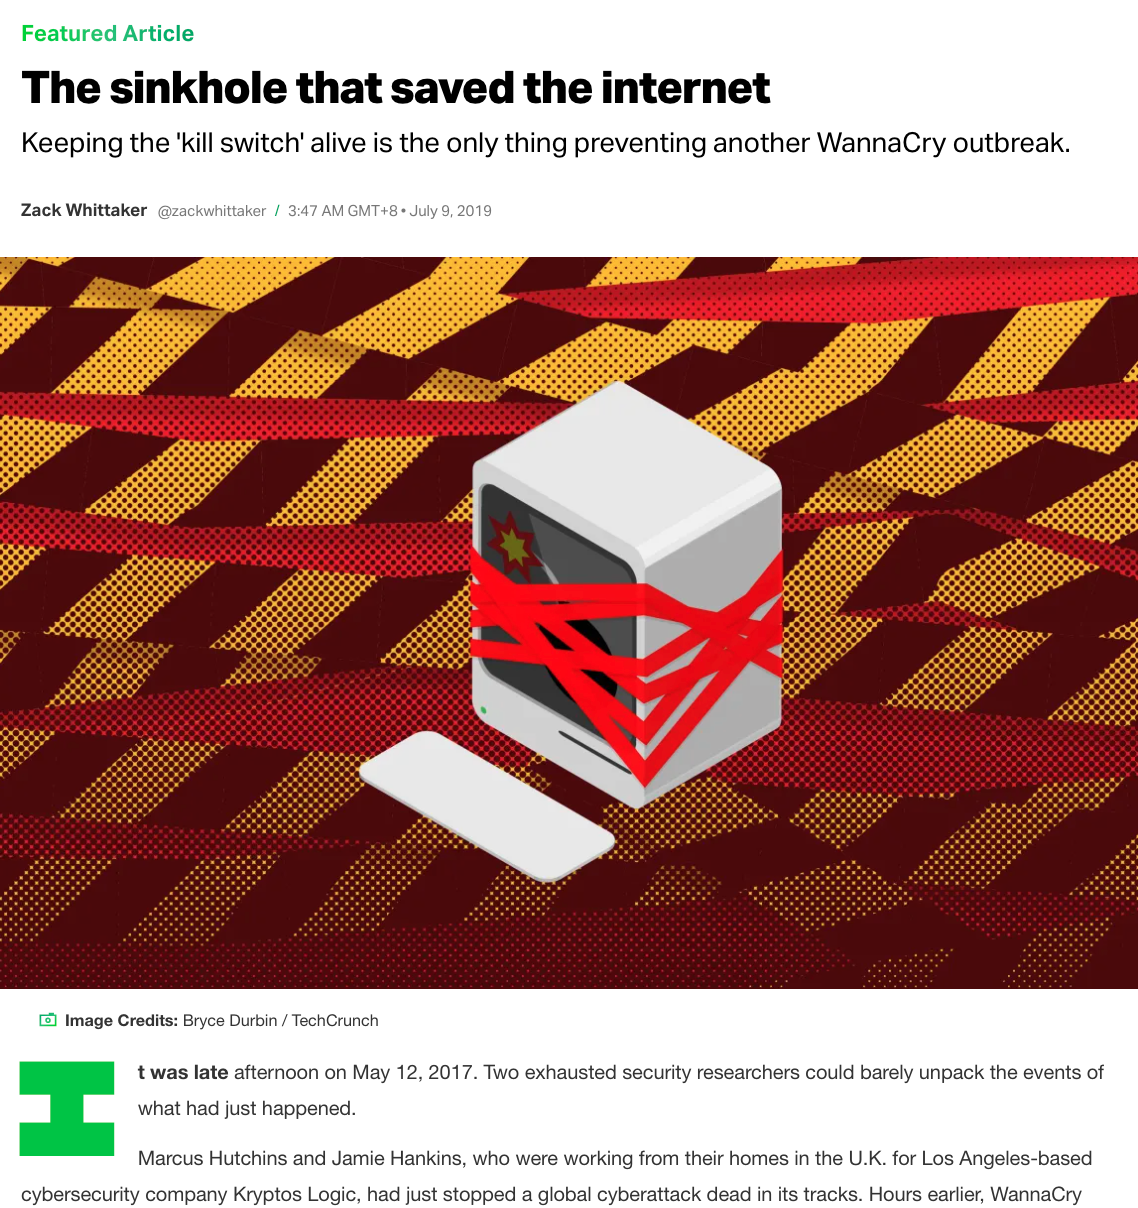
\includegraphics[height=0.95\textheight]{wannacry-news}
% \end{frame}


\section[Back to the Basics]{Back to the Basics\\\vspace{-5pt}{\tiny Early Stages of Reverse-Engineering Grief and Trauma}}
\frame{\sectionpage
    \begin{center}
        Early Stages of Reverse-Engineering Grief and Trauma
    \end{center}}


\subsection{COMP4901N Review}
\begin{frame}[fragile]{Symbolic Execution -- General Idea}
    \begin{columns}[t]
        \column{0.34\textwidth}
        \begin{block}{Code}
            \begin{lstlisting}[style=plainc,basicstyle=\tiny\ttfamily,gobble=16]
                void hello(uint8_t c) {
                    uint8_t win;
                    uint32_t a = c;
                    a = a*2 + 0xdeadbeef;
                    if (a >= 0 && a < 0xbaad)
                        win = 1;
                    else
                        win = 0;
                }
            \end{lstlisting}
        \end{block}
        \column{0.2\textwidth}
        \begin{block}{Concrete}
            \begin{lstlisting}[style=plain2,basicstyle=\tiny\ttfamily,gobble=16]
                c = 0xf0

                a = 0x000000f0
                a = 0xdeadc0cf


                
                win = 0
            \end{lstlisting}
        \end{block}
        \column{0.35\textwidth}
        \vskip-0.5pt % Why are they not aligned?
        \begin{block}<2->{Symbolic}
            \vskip-0.9pt % Why?
            \begin{lstlisting}[style=plain2,keywords={If,And,UGE,ULT,ZeroExt},basicstyle=\tiny\ttfamily,keywordstyle=\color{blue!80},gobble=16]
                <<c is an 8-bit input var>>

                a_0 = ZeroExt(24, c)
                a = a_0 * 2 + 0xdeadbeef
                win = If(And(UGE(a, 0),
                             ULT(a, 0xbaad)),
                         1,
                         0)
            \end{lstlisting}
        \end{block}
    \end{columns}
\end{frame}
\begin{frame}[fragile]{angr Level 1 -- Constrain your angr!}
    \begin{spacing}{0.95}
        \begin{lstlisting}[style=hybridpy,gobble=12]
            import angr
            from claripy import *

            @p = angr.Project('./level1')@
            @flag_bvs = [BVS(f'f_{i}', 8) for i in range(32)]@
            @state = p.factory.entry_state(
                        stdin=Concat(*flag_bvs, BVV('\n', 8)))@

            @for bv, ch in zip(flag_bvs, b'flag{'):
                state.solver.add(bv == BVV(ch, 8))

            for bv in flag_bvs:
                state.solver.add(bv >= BVV(0x20, 8))
                state.solver.add(bv <= BVV(0x7f, 8))@
                
            @simgr = p.factory.simgr(state)@
            @simgr.explore(find=0x40170f)@
            @print(simgr.found[0].posix.dumps(0))@
        \end{lstlisting}
    \end{spacing}
\end{frame}
\begin{frame}{angr Level 1 -- Constrain your angr!}
    \angrModelShowFlow{1}
\end{frame}
\begin{frame}{What's next?}
    \angrModelShowFlow{2}
\end{frame}


\section[Training Your angr]{Training Your angr\\\vspace{-5pt}{\tiny Wild \textbf{PRIMEAPE} used \textbf{RAGE}!}}
\frame{
    \vskip2em
    \sectionpage
    \begin{center}
        Wild \textbf{PRIMEAPE} used \textbf{RAGE}!
    \end{center}
    \vskip1em
    \begin{columns}
        \column{0.4\textwidth}
        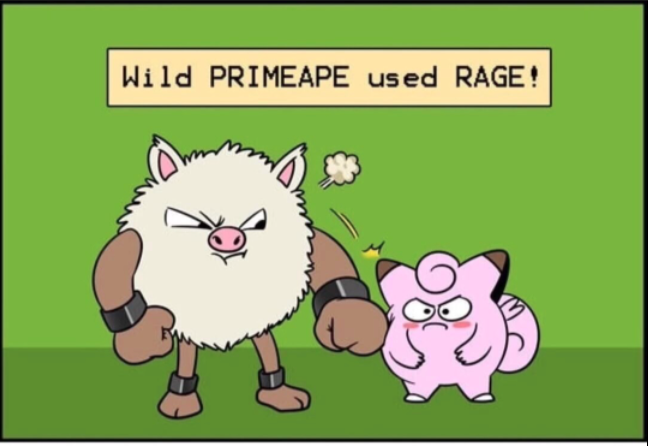
\includegraphics[width=\columnwidth]{primeape-rage-1}
        \column{0.4\textwidth}
        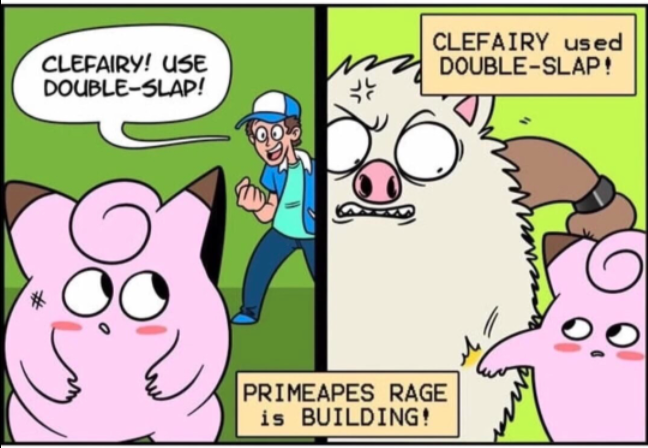
\includegraphics[width=\columnwidth]{primeape-rage-2}
    \end{columns}
}
\begin{frame}{Some Terminology}
    \begin{itemize}
        \item bitvector (BV): a sequence of bits
        \item symbol: unknown data {\scriptsize (Schrödinger's cat)}
        \item concrete: known data {\scriptsize (Schrödinger's cat outside the box)}
        \item concretise: process of [symbol $\arr$ concrete] w.r.t. constraints {\scriptsize (opening Schrödinger's box)}
        \item<2-> mixin: a design pattern promoting customisations (plugins)
    \end{itemize}
\end{frame}


\subsection{Concepts -- SimState}
\frame{
    \centering
    
\includegraphics[height=\textheight]{simstate-meme}
}
\begin{frame}[fragile]{SimState Concretisation}
    \begin{block}{\code{state.solver.eval(e, cast\_to=None)}}
        Evaluates (concretises) a bitvector and optionally casts to the type specified by \codec{cast\_to} (\codec{int} or \codec{bytes}).
    \end{block}
    \-\\
    \-\\
    \begin{block}{\code{state.posix.dumps(fd)}}
        Concretises and dumps stdin (0), stdout (1), or stderr (2) as bytes.
    \end{block}
    \morefootnote{https://docs.angr.io/core-concepts/solver#more-solving-methods}
    \absgraphic{
\includegraphics[height=0.15\textheight]{pooping}}[4.3cm][-5.0cm]
\end{frame}
\begin{frame}[fragile]{{\small A Tale of Two} SimState Memory Lanes}
    \begin{block}{DefaultMemory (Mixin Galore)}
        \begin{lstlisting}[style=plain2,gobble=12]
            state.memory.store(addr: int, data: int | bytes | BV)
            state.memory.load(addr: int, size: int) $\arr$ BV
        \end{lstlisting}
    \end{block}
    \begin{block}{SimMemView}
        \begin{lstlisting}[style=plain2,gobble=12]
            state.mem[<addr>].<type>.<resolved | concrete>
        \end{lstlisting}
    \end{block}
\end{frame}
\begin{frame}[fragile]{\code{state.memory}}
    \begin{lstlisting}[style=hybrid2,gobble=8]
        @state.memory.store(0x404000, b'/bin/sh\x00')@

        @bv = state.memory.load(0x404004, 4)
        state.solver.eval(bv, cast_to=bytes)@
        $\arr$ b'/sh\x00'
    \end{lstlisting}
    \begin{center}
        \begin{tikzpicture}[text height=1.5ex, text depth=0.25ex, yshift=0.5mm,minimum width=35pt,minimum height=25pt]
    \node[style=basic] (n0) {\footnotesize\texttt{/}};
    % Boxes.
    \foreach \x [count=\xi, remember=\xi as \lastxi (initially 0)] in {b,i,n,/,s,h,\textbackslash x00}{
            \node[style=basic, right=0cm of n\lastxi] (n\xi) {\footnotesize\texttt\x};
        }
    % Addresses.
    \foreach \x in {0,...,7}{
            \node[style=none, minimum height=5pt, above=0cm of n\x] (t\x) {\tiny\texttt 0x40400\x};
        }
    % BV.
    \node[style=none, below=0.2cm of n7] (bv) {\footnotesize\code{<BV8 47>}};
    \draw[style=one-way arrow]
    (n4)
    to[bend right, out=-80, in=-180]
    node[below left=-0.3cm and 0.6cm]{
        \footnotesize\code{state.memory.load(0x404004, 1)}}
    (bv);
\end{tikzpicture}
    \end{center}

    \absfootnoteb{Byte order depends on endianness! Check \codec{state.arch}!}
    \morefootnote{https://docs.angr.io/core-concepts/states#low-level-interface-for-memory}
\end{frame}
\begin{frame}[fragile]{\code{state.mem}}
    \begin{lstlisting}[style=hybrid2,gobble=8]
        @state.mem[0x404000].uint32_t = 0x41424344@
        
        @state.mem[0x404000].uint16_t.resolved@
        $\arr$ <BV16 0x4344>

        @state.mem[0x404000].uint16_t.concrete@
        $\arr$ 0x4344
    \end{lstlisting}
    \begin{center}
        \begin{tikzpicture}[text depth=0.25ex, yshift=0.5mm,minimum width=35pt,minimum height=25pt]
    \node[style=basic] (n0) {\footnotesize\texttt{0x44}};
    % Boxes.
    \foreach \x [count=\xi, remember=\xi as \lastxi (initially 0)] in {0x43,0x42,0x41}{
            \node[style=basic, right=0cm of n\lastxi] (n\xi) {\footnotesize\texttt\x};
        }
    % Addresses.
    \foreach \x in {0,...,3}{
            \node[style=none, minimum height=5pt, above=0cm of n\x] (t\x) {\tiny\texttt 0x40400\x};
        }
    \node[right=0.2cm of n3, anchor=west] (text) {(Little Endian)};
    % % BV.
    % \node[style=none, align=center] (bv) at (5, -1) {\footnotesize\code{<uint16\_t <BV16 0x4344> at 0x404000>}};
    
    % \draw[style=one-way arrow]
    % (n0.south east) + (0,-0.1cm)
    % to[bend right, out=-60, in=-175]
    % node[below left=-0.25cm and -0.2cm]{
    %     \tiny\code{state.mem[0x404000].uint16\_t}}
    %     (bv);

    % \node[style=none] (resolved) at (3.5,-2.3) {\footnotesize\code{<BV16 0x4344>}};
    % \node[style=none] (concrete) at (6.5,-2.3) {\footnotesize\code{0x4344}};
    % \draw[style=one-way arrow] (bv) to node[left=0.2cm]{\tiny\code{.resolved}} (resolved);
    % \draw[style=one-way arrow] (bv) to node[right=0.2cm]{\tiny\code{.concrete}} (concrete);

\end{tikzpicture}
    \end{center}
    \absfootnote{Byte order depends on endianness! Check \codec{state.arch}!}
\end{frame}
\begin{frame}{\code{state.mem}}
    \begin{center}
        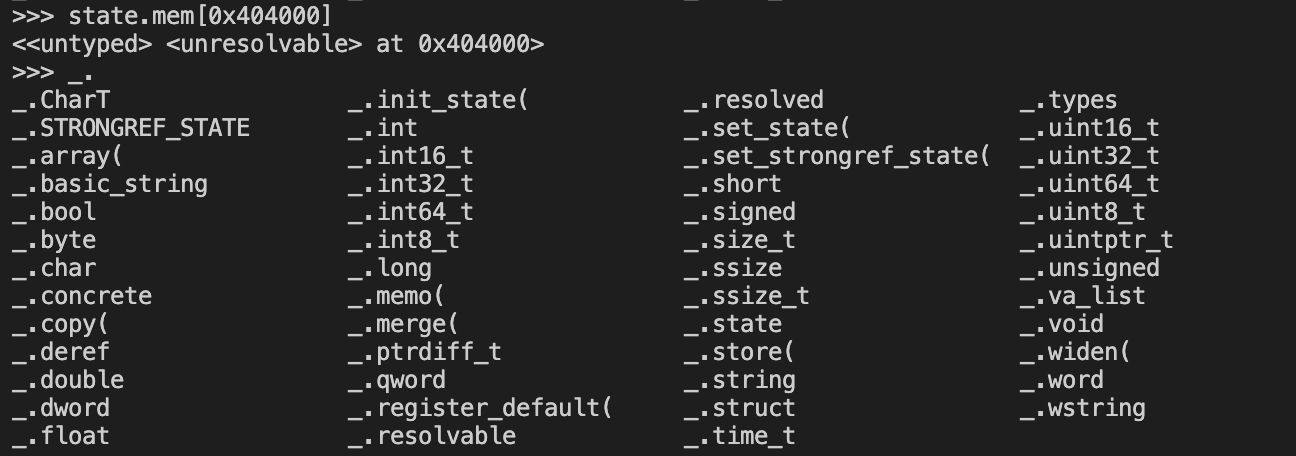
\includegraphics[width=\textwidth]{state-mem}
    \end{center}
    \absfootnote{Note: some types are not available for some arches (e.g. no \codec{int64\_t} for 32-bit arches).}
\end{frame}
\begin{frame}[fragile]{\code{state.regs}}
    \begin{lstlisting}[style=plain2,gobble=8]
        state.regs.pc
        $\arr$ <BV64 0x4011c8>
    \end{lstlisting}
    \vspace{-10pt}
    \begin{center}
        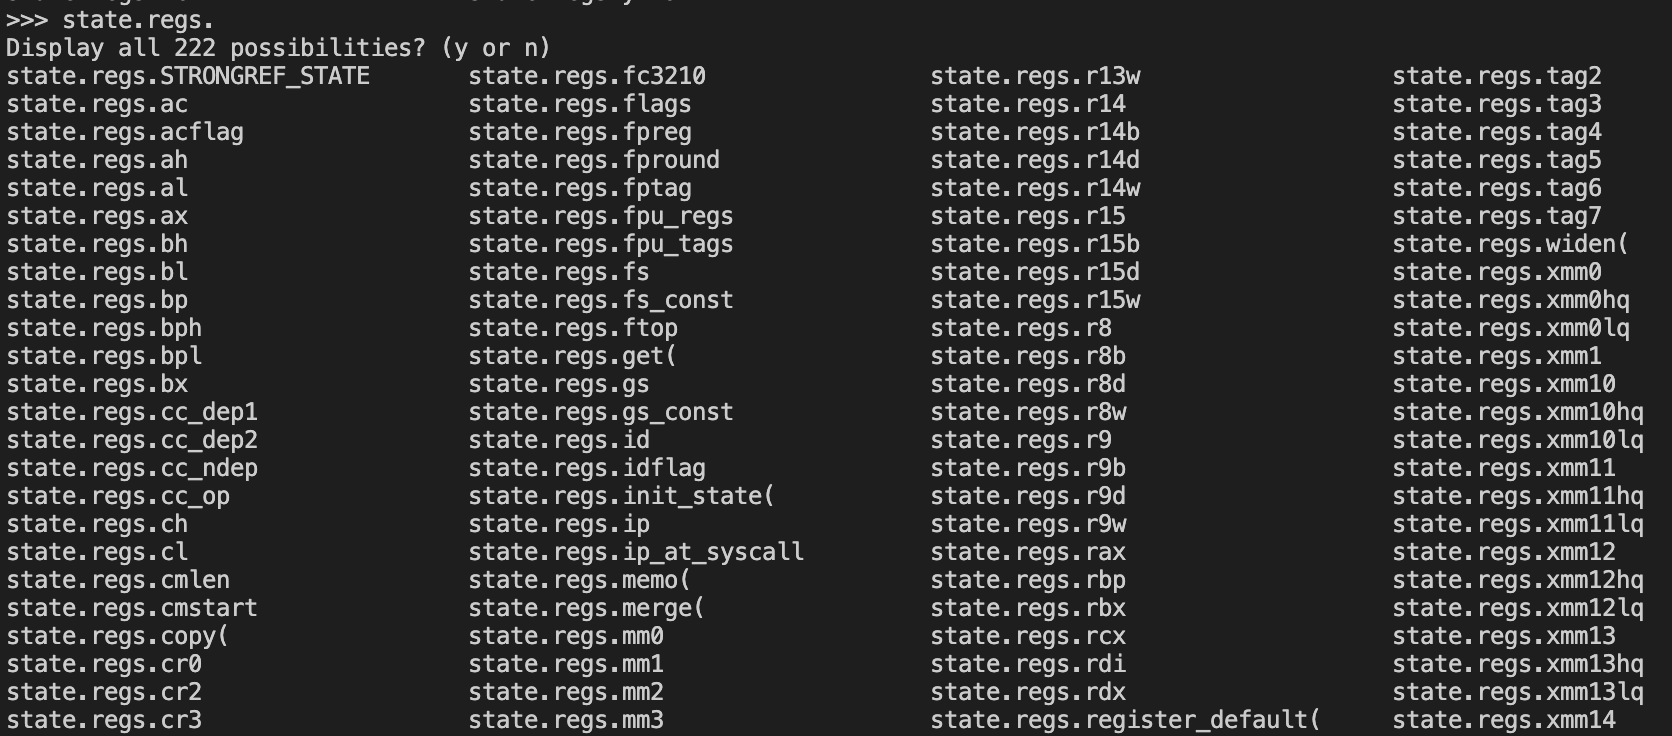
\includegraphics[width=\textwidth]{state-regs}
    \end{center}
    \absfootnote{Not all completions are shown.}
\end{frame}


\subsection{Concepts -- Simulation Manager}
% \frame{
%     \subsectionpage
% }
\begin{frame}[fragile]{\code{simgr.explore\small(find, avoid, n, num\_find, ...)}}
    Simulate until constraints are met (or until no more states could be stepped).
    \begin{itemize}
        \item<2-> \codec{find}{\small\lstinline{:  int | [int] | (SimState $\arr$ bool) = None}}
        \item<2-> \codec{avoid}{\small\lstinline{: int | [int] | (SimState $\arr$ bool) = None}}
              \begin{itemize}
                  \item An address, a list of addresses, or a predicate which takes a state and returns whether it should be marked found/avoided (\codec{return True}) or continue to be active (\codec{return False}).
              \end{itemize}
        \item<3-> \codec{n}{\small\lstinline{: int = None}}
              \begin{itemize}
                  \item Number of steps to advance. If \codec{None}, run until other conditions are met.
              \end{itemize}
        \item<3-> \codec{num\_find}{\small\lstinline{: int = 1}}
              \begin{itemize}
                  \item Number of states to look for in the \codec{`found'} stash.
              \end{itemize}
    \end{itemize}
\end{frame}
\begin{frame}[fragile]{\code{simgr.stashes\small[...]}}
    Where are the simulated states?
    \begin{itemize}
        \item<2-> \codec{`active'}: States here are alive and well.
        \item<2-> \codec{`found'}: States here match search criteria and constraints.
        \item<3-> \codec{`deadended'}: States finished executing or can't continue.
              \begin{itemize}
                  \item Possible causes: \codec{exit(n)}, no more sat states, program crashed (invalid instruction, memory access, etc.).
                  \item ``Why did my state deadend?'' See \slideref{debugging-states} to see where to start debugging!
              \end{itemize}
        \item<4-> \codec{`errored'}: States that terminated due to a Python exception (simulation error, claripy error, etc.).
    \end{itemize}

    \absfootnoteb{Note: \codec{simgr.stashes[`active']}\code{ == }\codec{simgr.active}.}
    \morefootnote{https://docs.angr.io/core-concepts/pathgroups#stash-types}
\end{frame}


\subsection{SOMP1010: angr Management -- Midterm}
\frame{
    \subsectionpage
    \absgraphic{
\includegraphics[width=3cm]{fat-shiba-shock}}[0.5cm][-6cm]
}
\begin{frame}{Q1 -- Address?}
    \begin{center}
        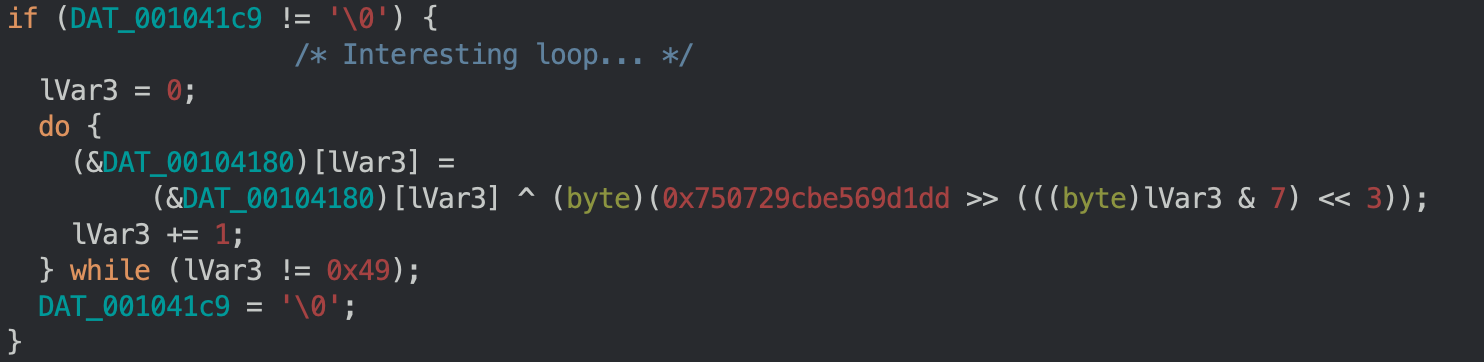
\includegraphics[width=\textwidth]{tooling-q2}
    \end{center}
    \vspace{-0.2em}
    \begin{block}<2->{What is the address of the secret?}
        \vskip0.4em
        \begin{enumerate}[(A)]
            \item<beamer:alert@3> 0x104180
            \item 0x1041c9
            \item 0x49
            \item 0x750729cbe569d1dd
        \end{enumerate}
    \end{block}
\end{frame}
\begin{frame}{Q2 -- Length?}
    \begin{center}
        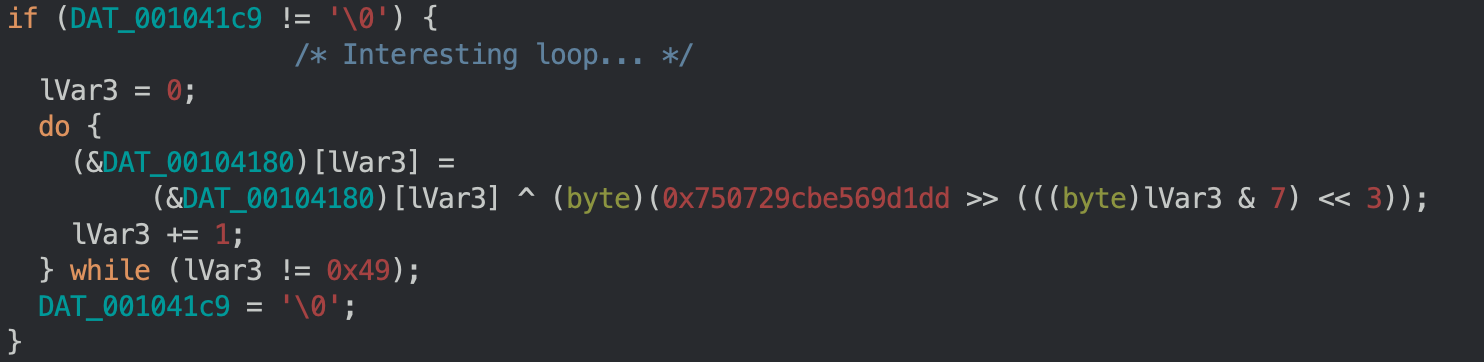
\includegraphics[width=\textwidth]{tooling-q2}
    \end{center}
    \vspace{-0.2em}
    \begin{block}{What is the length of the secret?}
        \vskip0.4em
        \begin{enumerate}[(A)]
            \item<beamer:invisible> 1
            \item 0x48
            \item<beamer:invisible> 49
            \item<beamer:invisible> 0x49
        \end{enumerate}
    \end{block}
    % \absfootnote{Hint: the length of \codec{b`a\textbackslash x00'} is 1.}
\end{frame}
\begin{frame}[fragile]{Q3 -- How to print?}
    \begin{lstlisting}[style=plainpy,gobble=8]
        simgr = p.factory.simgr()
        simgr.explore(find=0x401206)
        s = simgr.found[0]
    \end{lstlisting}
    \begin{block}{Which of the following correctly concretises and prints out the secret (assuming there are no null bytes in the 72 characters)?}
        \vskip0.4em
        \begin{enumerate}[(A)]
            \item<beamer:alert@2> {\scriptsize\code{s.mem[0x404180].string.concrete}}
            \item<beamer:alert@2> {\scriptsize\code{s.solver.eval(s.memory.load(0x404180, 72), cast\_to=bytes)}}
            \item<beamer:alert@2> {\scriptsize\code{b`'.join(s.mem[0x404180+i].char.concrete for i in range(72))}}
        \end{enumerate}
    \end{block}

    \absfootnoteb{Note: tooling is a PIE binary. By default, ghidra and angr loads PIE binaries at a base address of 0x100000 and 0x400000 respectively; so by default, 0x101234 in ghidra == 0x401234 in angr.}
\end{frame}
\frame{
    \centering
    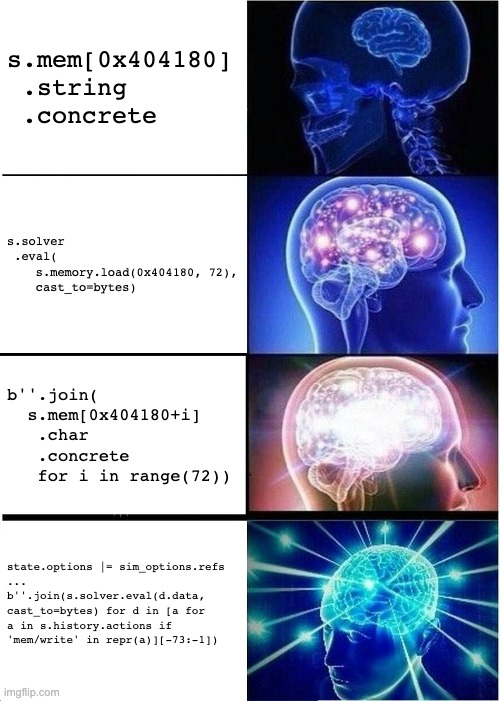
\includegraphics[height=\textheight]{tooling-bigbrain}
}
\subsection{Training Summary}
\begin{frame}{Summary}
    \angrModelShowFlow{2}
\end{frame}
\begin{frame}{But wait-- there's more!}
    \angrModelShowFlow{3}
\end{frame}
\begin{frame}[fragile]{But wait-- there's more!}
    \small
    \begin{itemize}
        \item \exref{https://docs.angr.io/core-concepts/loading}{\code{cle.Loader}}: options to load x86, AVR, MIPS, etc. instructions from binary, Intel hex, etc. into an unified interface.
        \item \exref{https://docs.angr.io/core-concepts/states#state-presets}{State Presets}: start simulating from the beginning of an arbitrary function or point in code.
        \item \exref{https://docs.angr.io/core-concepts/pathgroups#exploration-techniques}{\code{exploration\_techniques}}: different ways to explore paths, keep track of states, etc.
        \item \exref{https://docs.angr.io/extending-angr/simprocedures}{Hooks and \code{SimProcedure}s}: attach your own emulation code to functions/callbacks.
        \item \exref{https://docs.angr.io/core-concepts/states#state-options}{\code{state.options}}: fine-tune the simulation and solver engines.
        \item \exref{https://docs.angr.io/core-concepts/simulation}{Execution Engine}: customise which mixins are used to process instructions.
    \end{itemize}
\end{frame}


\subsection{What's next?}
\begin{frame}<handout:0>{What's next?}
    \angrModelShowFlow{3}
\end{frame}
\begin{frame}[noframenumbering]{What's next?}
    \angrModelShowFlow{4}
\end{frame}

\subsection{}
\begin{frame}{Questions?}
    \centering
    
\includegraphics[width=0.8\textwidth]{questions-2}
\end{frame}


\section[Analysis with angr -- CFGs]{Analysing with angr -- CFGs\\\vspace{-5pt}{\tiny Investigating the Behavioural Economics of Machine Code}}
\frame{
    \vskip2em
    \sectionpage
    \begin{center}
        Investigating the Behavioural Economics of Machine Code
    \end{center}
    \vskip1em
    \begin{columns}
        \column{0.4\textwidth}
        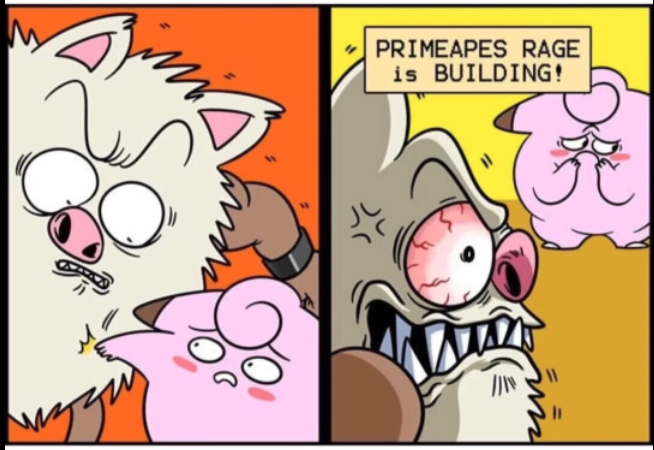
\includegraphics[width=\columnwidth]{primeape-rage-3}
        \column{0.4\textwidth}
        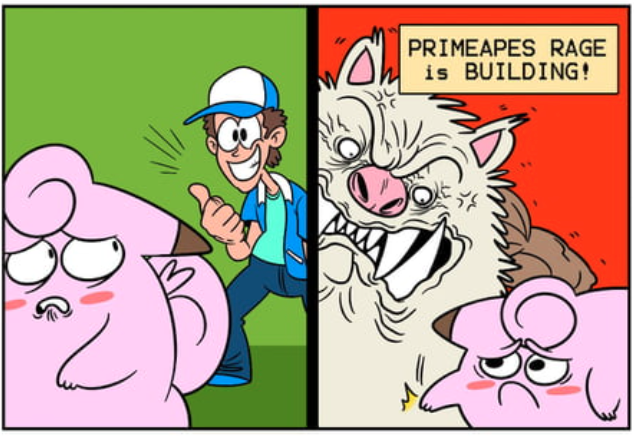
\includegraphics[width=\columnwidth]{primeape-rage-4}
    \end{columns}
}
\begin{frame}{An Appetiser}
    \centering
    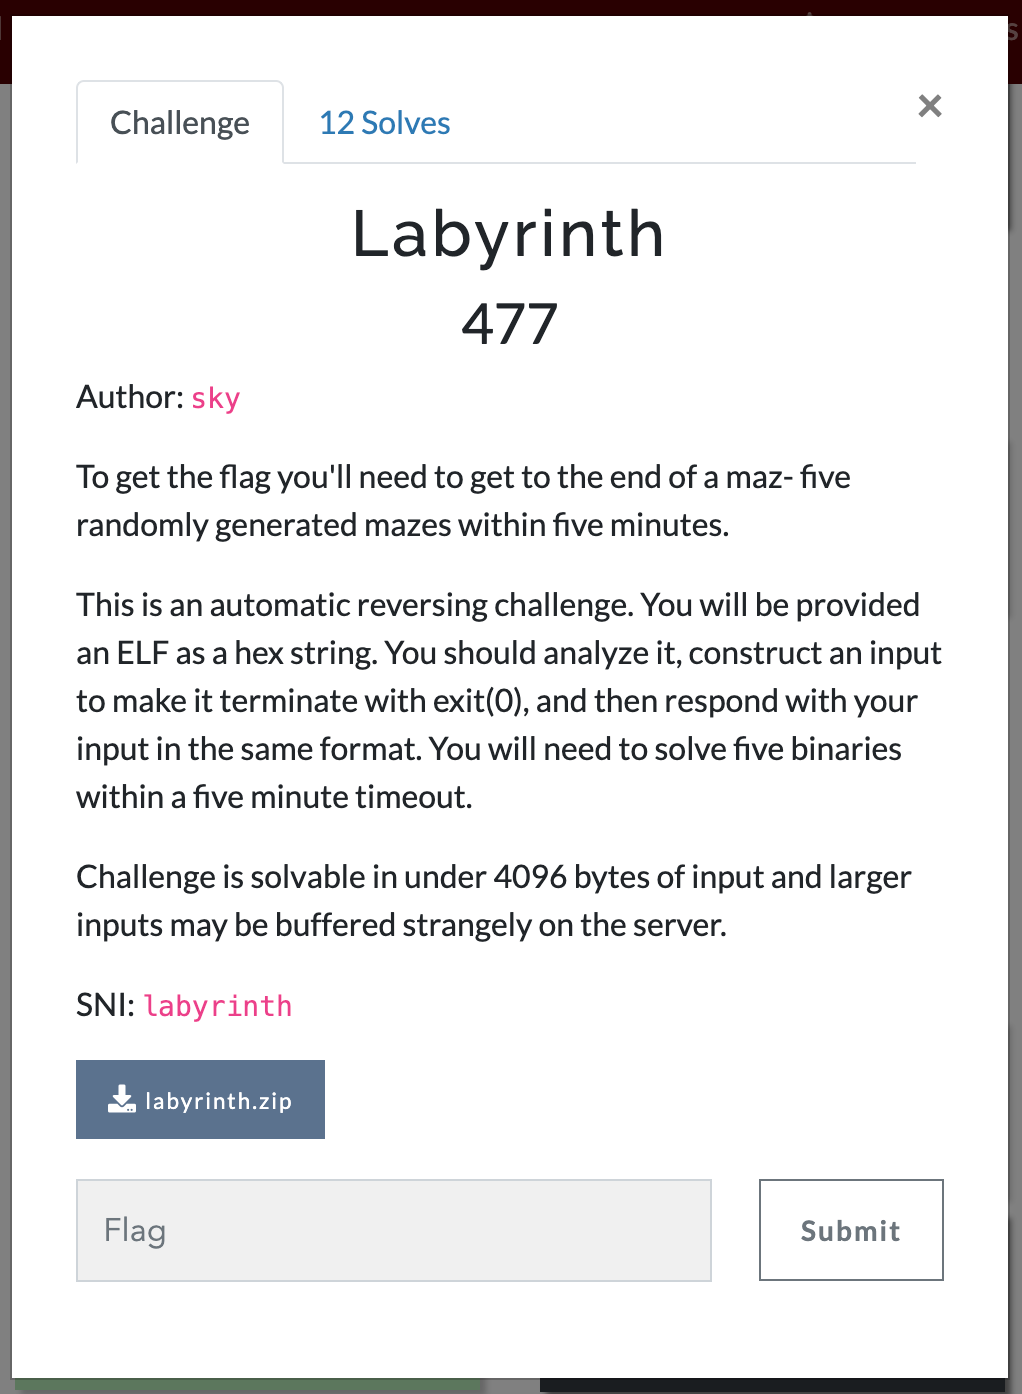
\includegraphics[height=0.9\textheight]{chal-labyrinth}
\end{frame}
\begin{frame}{Gru's Plan}
    \centering
    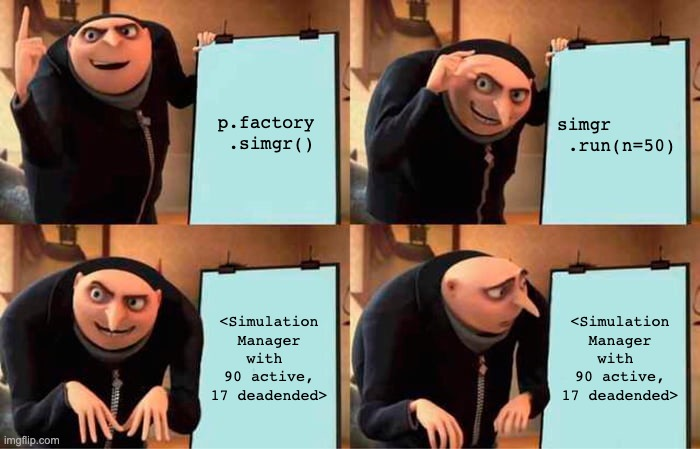
\includegraphics[height=0.9\textheight]{path-explosion-gru}
\end{frame}
\subsection{What went wrong?}
\begin{frame}{What went wrong?}
    \centering
    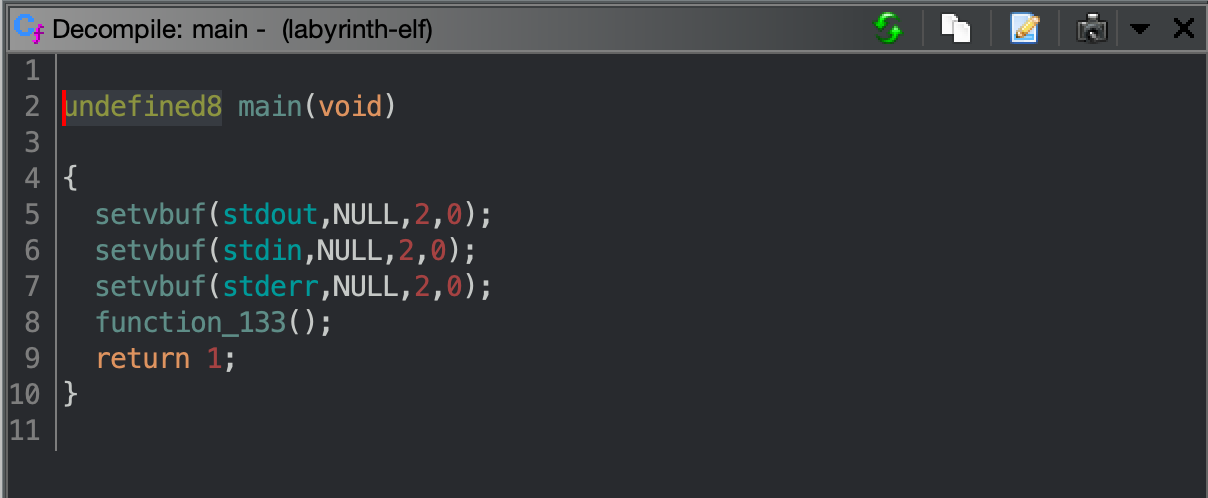
\includegraphics[scale=0.45]{labyrinth-1}
\end{frame}
\begin{frame}{What went wrong?}
    \centering
    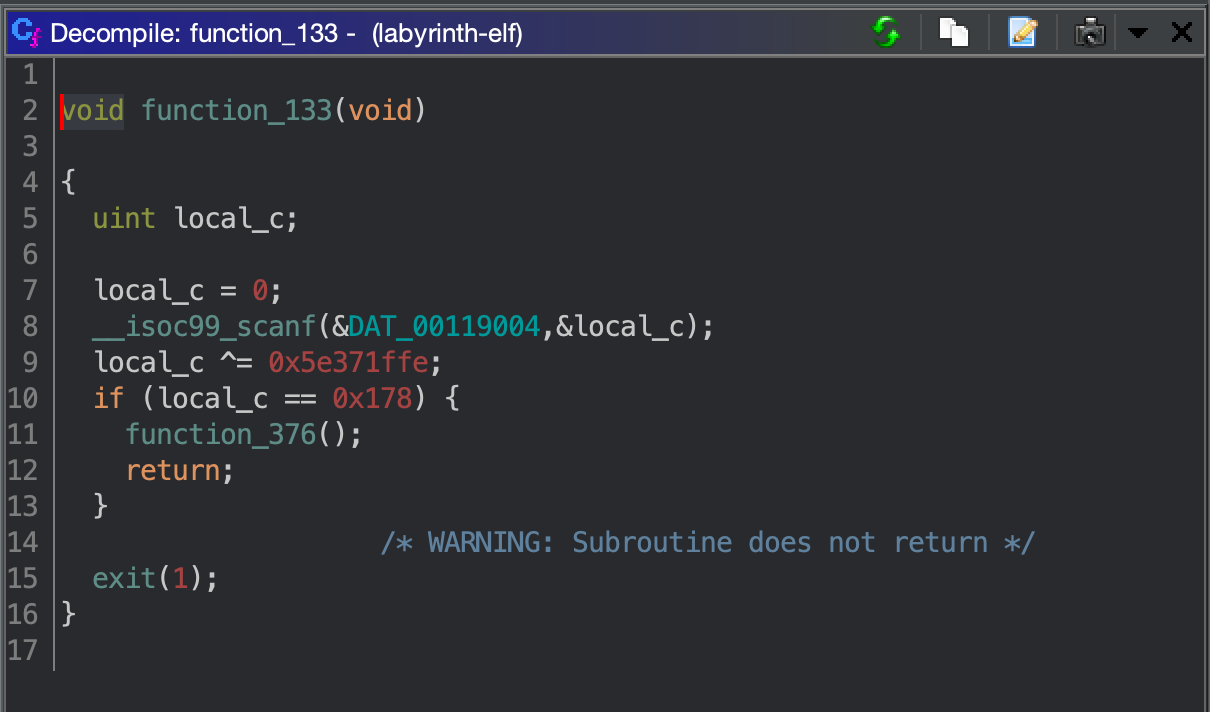
\includegraphics[scale=0.45]{labyrinth-2}
\end{frame}
\begin{frame}{What went wrong?}
    \centering
    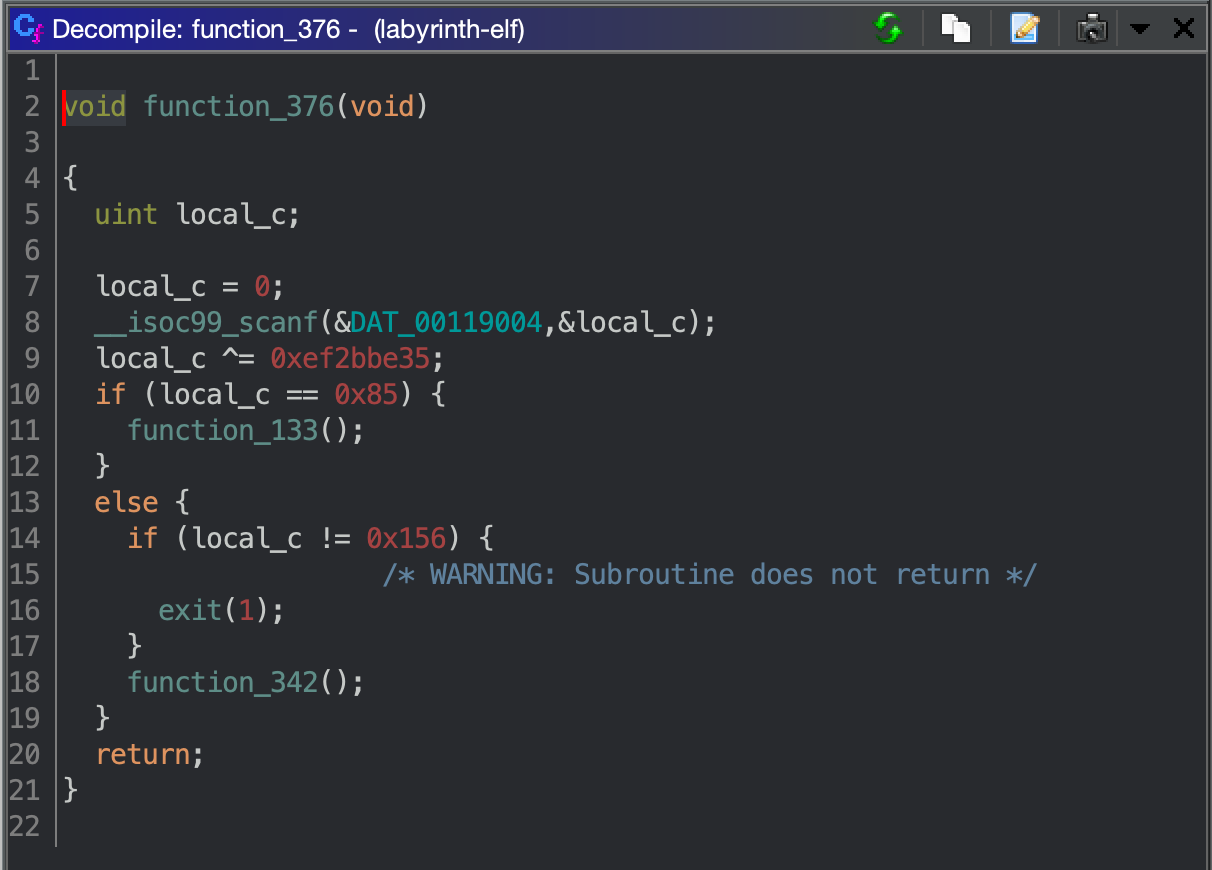
\includegraphics[scale=0.45]{labyrinth-3}
    \begin{uncoverenv}<2->
        \begin{tikzpicture}[overlay]
            \node[text=red] (txt) at (-3, 3.5) {Repeats!};
            \draw[style=one-way arrow, color=red] (txt) to (-6.7, 3.5);
        \end{tikzpicture}
    \end{uncoverenv}
\end{frame}
\begin{frame}{Path Explosion}
    \ctikzfig{labyrinth-path-explosion}
\end{frame}
\begin{frame}{Path Explosion}
    \begin{columns}
        \column{0.4\textwidth}
        
\includegraphics[width=\columnwidth]{path-explosion-1}
        \column<2->{0.4\textwidth}
        
\includegraphics[width=\columnwidth]{path-explosion-2}
        \column<3->{0.4\textwidth}
        
\includegraphics[width=\columnwidth]{path-explosion-3}
    \end{columns}
\end{frame}
% \begin{frame}{Who's that pokemon?}
%     \centering
%     
\includegraphics[width=0.8\textwidth,clip,trim=6cm 0 6cm 0]{who-cfg}
% \end{frame}
% \begin{frame}{It's CFG!}
\begin{frame}{Control Flow Graphs to the Rescue}
    \centering
    
\includegraphics[width=0.8\textwidth]{cfg-squirtle}
\end{frame}


\subsection{MATH2343/COMP2711 Review}
\begin{frame}{G-raph?}
    \centering
    
\includegraphics[height=0.9\textheight]{graph}
    \absgraphic{
\includegraphics[height=0.3\textheight]{stonks}}[1cm][-3cm]
\end{frame}
\begin{frame}{Graphs}
    \ctikzfig{graph-simple}
\end{frame}
\begin{frame}{G-raph!}
    \centering
    
\includegraphics[height=0.9\textheight]{graph}
    \begin{textblock}{5}(4,5)
        \tikzfig{graph-melman}
    \end{textblock}
\end{frame}
\begin{frame}{Graphs}
    \centering
    \includegraphics[width=0.85\textwidth]{graph2}
    \begin{textblock}{5}(1.7,3.65)
        \tikzfig{graph-hkust}
    \end{textblock}
\end{frame}
\begin{frame}{Graphs}
    \centering
    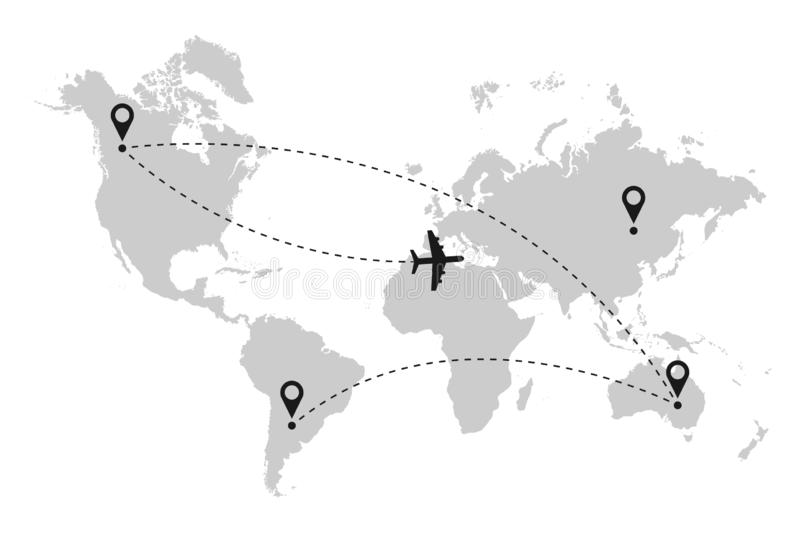
\includegraphics[width=0.85\textwidth]{graph-flight}
    \begin{textblock}{5}(4.65,6.8)
        \tikzfig{graph-flight}
    \end{textblock}
\end{frame}


\subsection{Control Flow Graphs}
\begin{frame}{Programs as Graphs}
    \ctikzfig{labyrinth-path-explosion}
\end{frame}
\begin{frame}{Programs as Graphs}
    \ctikzfig{labyrinth-path-explosion-1}
\end{frame}
\begin{frame}{Programs as Graphs}
    \ctikzfig{labyrinth-path-explosion-2}
\end{frame}
\begin{frame}{Programs as Graphs}
    \ctikzfig{labyrinth-path-explosion-3}
\end{frame}
\begin{frame}{What about branches and loops?}
    \ctikzfig{labyrinth-path-explosion-4}
    \absgraphic{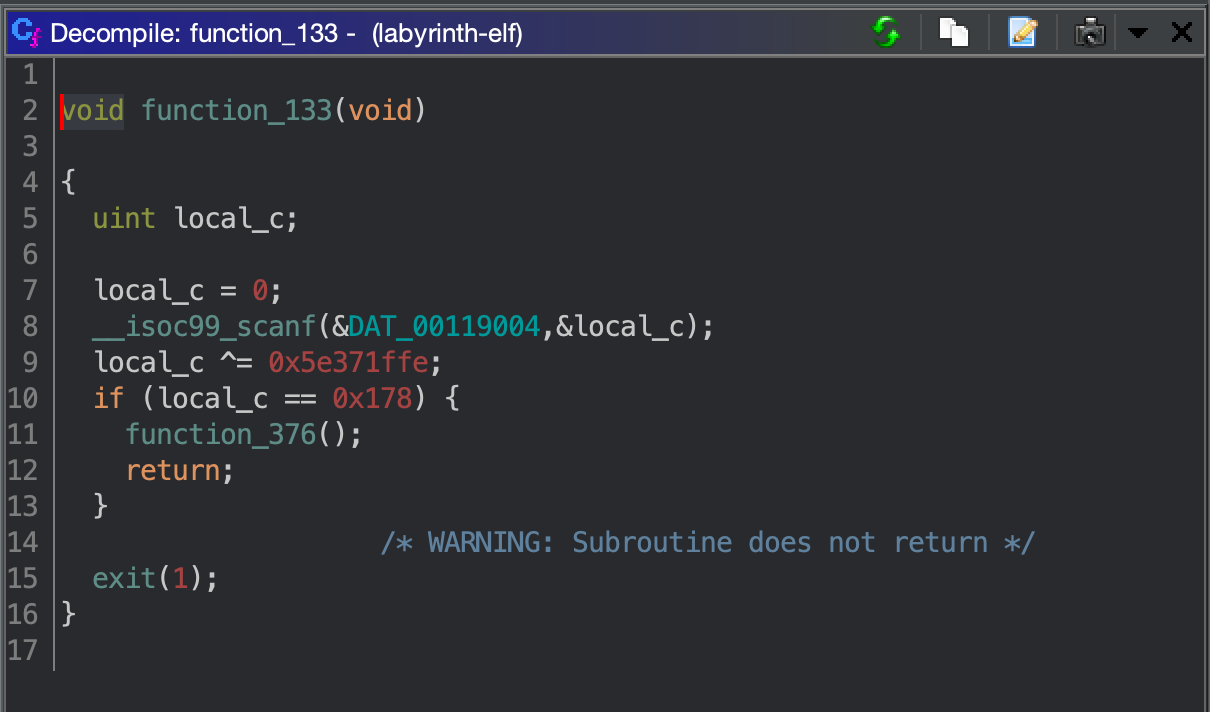
\includegraphics[scale=0.35,clip,trim=0 0 1cm 1.5cm]{labyrinth-2}}[6.5cm][-6cm]
\end{frame}
\begin{frame}<handout:0>{Do you recognise these CFGs?}
    \centering
    \resizebox{!}{0.9\height}{\tikzfig{cfg-1}}
\end{frame}
\begin{frame}[noframenumbering]{Do you recognise these CFGs?}
    \centering
    \resizebox{!}{0.9\height}{\tikzfig{cfg-1a}}
\end{frame}
\begin{frame}<handout:0>{Do you recognise these CFGs?}
    \centering
    \resizebox{!}{0.9\height}{\tikzfig{cfg-2}}
\end{frame}
\begin{frame}[noframenumbering]{Do you recognise these CFGs?}
    \centering
    \resizebox{!}{0.9\height}{\tikzfig{cfg-2a}}
\end{frame}
\begin{frame}<handout:0>{Do you recognise these CFGs?}
    \centering
    \resizebox{!}{0.9\height}{\tikzfig{cfg-3}}
\end{frame}
\begin{frame}[noframenumbering]{Do you recognise these CFGs?}
    \centering
    \resizebox{!}{0.9\height}{\tikzfig{cfg-3a}}
\end{frame}
\begin{frame}[fragile]{CFGs in angr}
    \begin{columns}[t]
        \column{0.45\textwidth}
        \begin{block}{{\scriptsize\code{p.analyses\\.}}\code{CFGFast}}
            \vskip0.4em
            \begin{itemize}
                \item<2-> static
                \item<3-> faster
                \item<4-> can analyse basic jumps
            \end{itemize}
        \end{block}
        \column{0.45\textwidth}
        \begin{block}{{\scriptsize\code{p.analyses\\.}}\code{CFGEmulated}}
            \vskip0.4em
            \begin{itemize}
                \item<2-> dynamic
                \item<3-> slower
                \item<4-> can analyse more obscure/hidden jumps, with context
            \end{itemize}
        \end{block}
    \end{columns}
    \-\\
    \-\\
    \begin{uncoverenv}<5->
        Class parameters? Check the \exref{https://docs.angr.io/built-in-analyses/cfg}{docs} + source code!
    \end{uncoverenv}
\end{frame}

\subsection{Demo}
\begin{frame}<handout:0>{Demo -- Labyrinth}
    \centering
    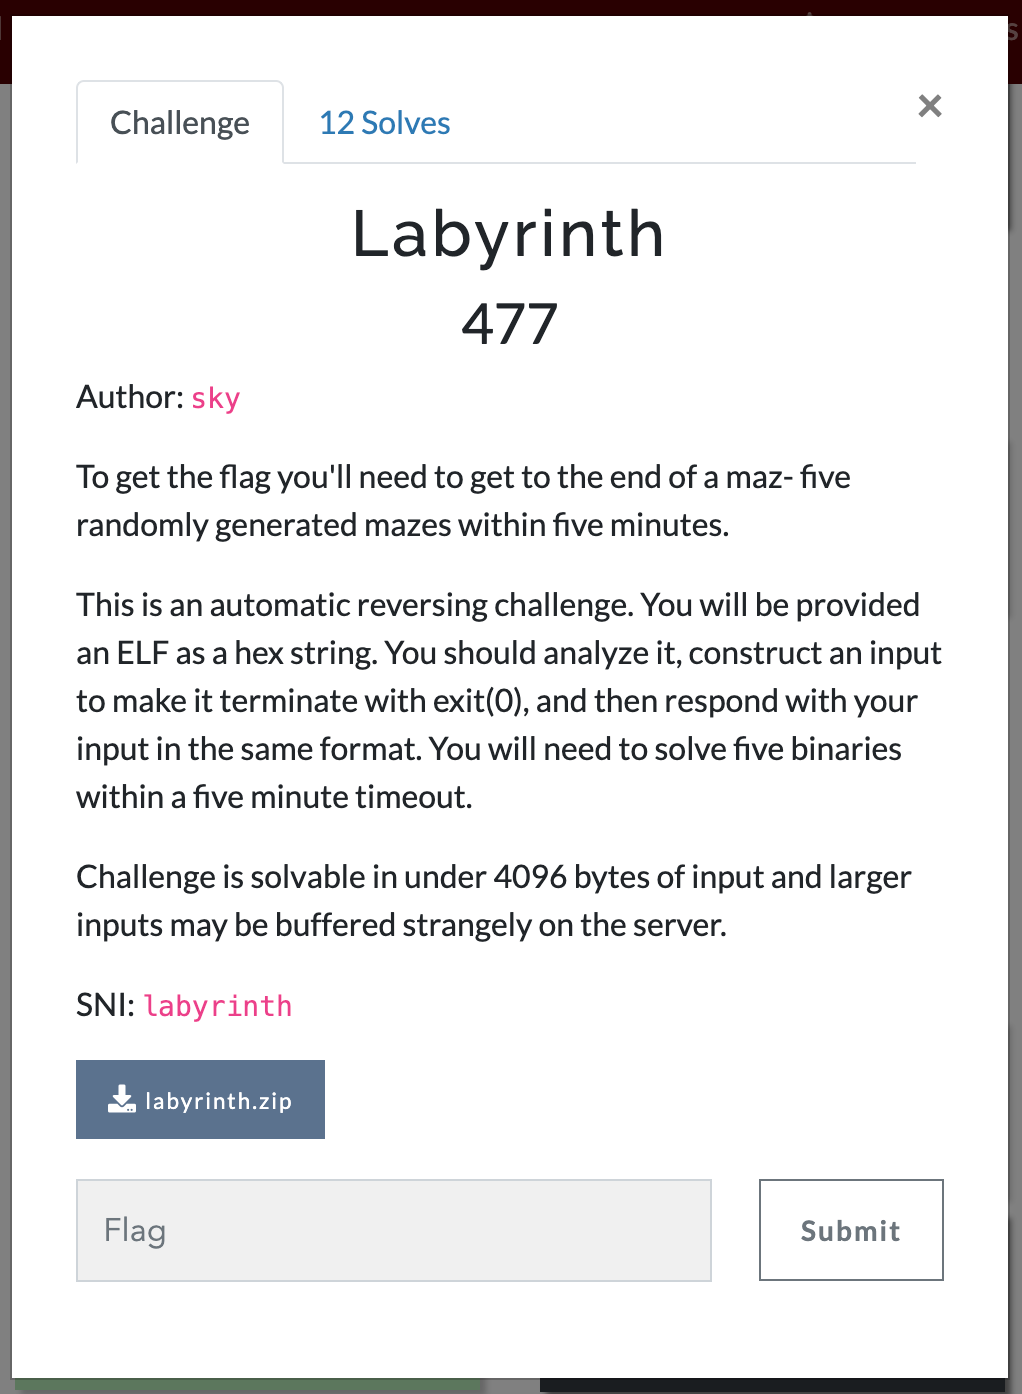
\includegraphics[height=0.9\textheight]{chal-labyrinth}
\end{frame}
\begin{frame}[noframenumbering]{Demo -- Labyrinth}
    \centering
    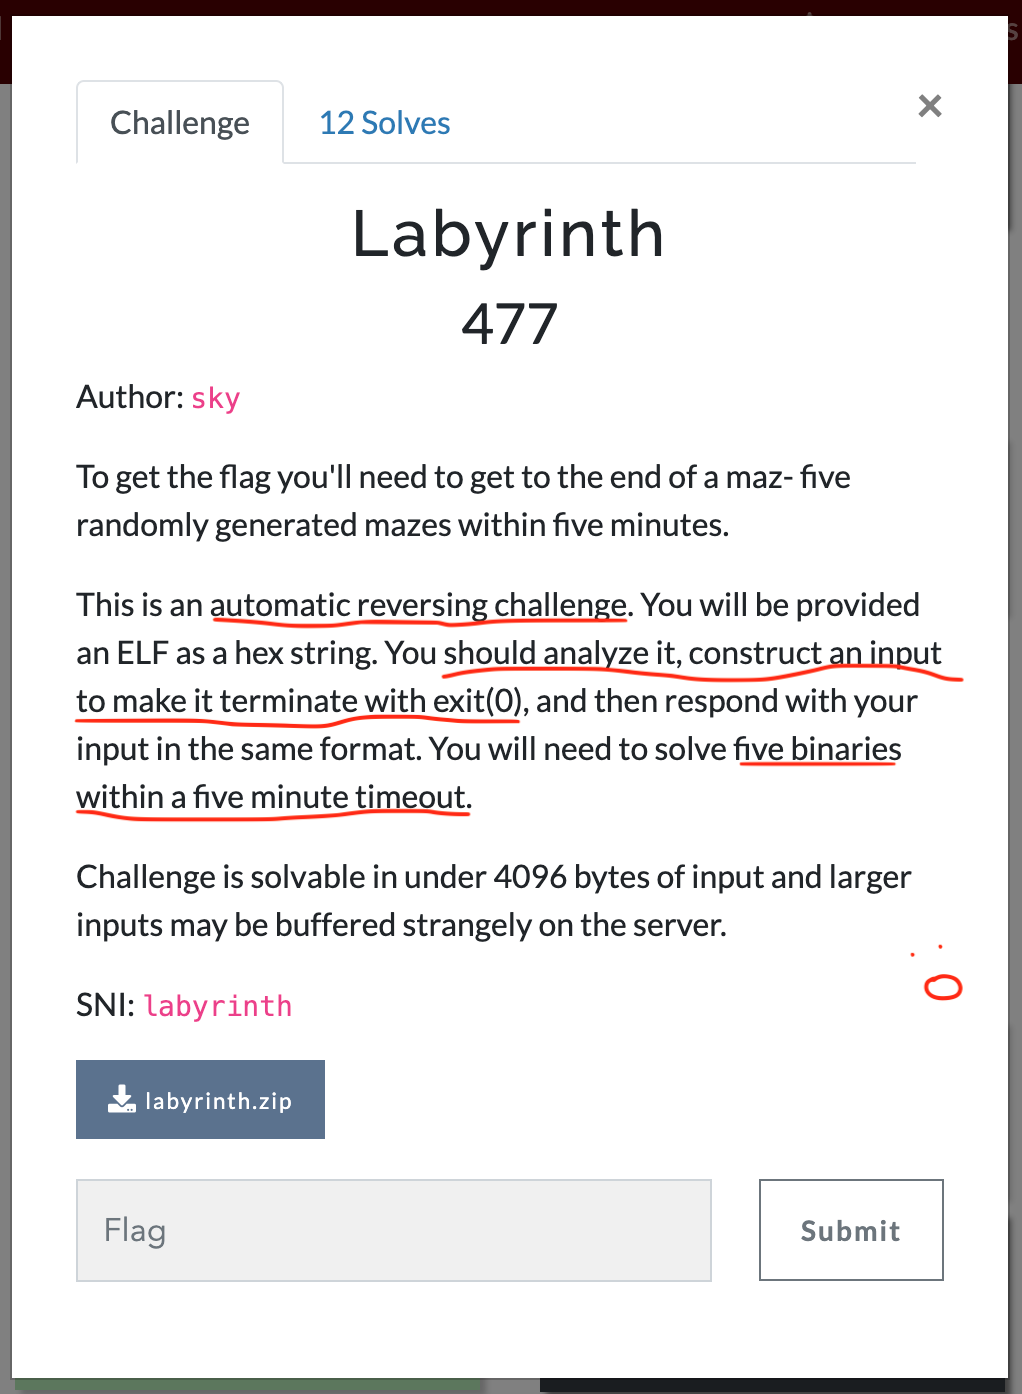
\includegraphics[height=0.9\textheight]{chal-labyrinth-annotated}
\end{frame}
\begin{frame}{Summary -- Labyrinth}
    \begin{enumerate}
        \item<1-> Load project
        \item<2-> Construct CFG (\codec{p.analyses.CFGFast})
        \item<3-> Get `from' and `to' nodes (\codec{main}, \codec{exit(0)})
        \item<3-> Construct shortest path (\codec{networkx.shortest\_path})
        \item<3-> Follow shortest path
        \item<4-> Take a dump
        \item<4-> Profit!
    \end{enumerate}
\end{frame}

\subsection{Analysis Summary}
\begin{frame}[fragile]{But wait-- there's moar!}
    \begin{block}<1->{Fun with CFGs}
        \begin{itemize}
            \item Reachability
            \item Compiler Optimisations
        \end{itemize}
    \end{block}
    \begin{block}<2->{Moar Analyses}
        \begin{itemize}
            \item<2-> Value Flow Graph (VFG), Value Set Analysis (VSA)
                  \begin{itemize}
                      \item What values can this variable hold?
                      \item CFGs are to instructions as VFGs are to data.
                  \end{itemize}
            \item<3-> Data Dependency Graph (DDG)
                  \begin{itemize}
                      \item What statements does this variable depend on?
                  \end{itemize}
            \item<4-> Moar!
        \end{itemize}
    \end{block}
    \morefootnote[Moar]{https://docs.angr.io/core-concepts/analyses}
\end{frame}
\begin{frame}<handout:0>{What's next?}
    \angrModelShowFlow{4}
\end{frame}
\begin{frame}[noframenumbering]{What's next?}
    \angrModelShowFlow{5}
\end{frame}

\subsection{}
\begin{frame}{Questions?}
    \centering
    
\includegraphics[width=0.8\textwidth]{questions-3}
\end{frame}


\section[Debugging angr Programs]{Debugging angr Programs\\\vspace{-5pt}{\tiny Towards Enhanced Emotional Resilience and Cognizance}}
\frame{
    \vskip2em
    \sectionpage
    \begin{center}
        Towards Enhanced Emotional Resilience and Cognizance
    \end{center}
    \vskip1em
    \begin{columns}
        \column{0.4\textwidth}
        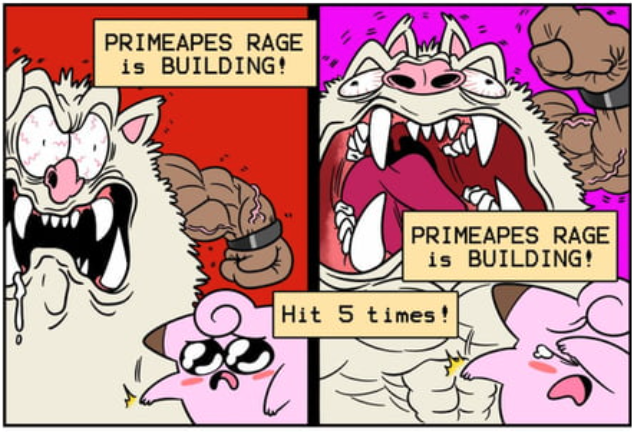
\includegraphics[width=\columnwidth]{primeape-rage-5}
        \column{0.4\textwidth}
        
\includegraphics[width=\columnwidth]{primeape-rage-6}
    \end{columns}
}

\subsection{Housekeeping}
\begin{frame}[fragile]{\code{logging}}
    \begin{lstlisting}[style=hybridpy,gobble=8]
        import logging
        
        @logging.getLogger('angr')
               .setLevel(logging.INFO)@

        @logging.getLogger('angr.analyses.cfg')
               .setLevel(logging.DEBUG)@
    \end{lstlisting}
    \begin{center}
        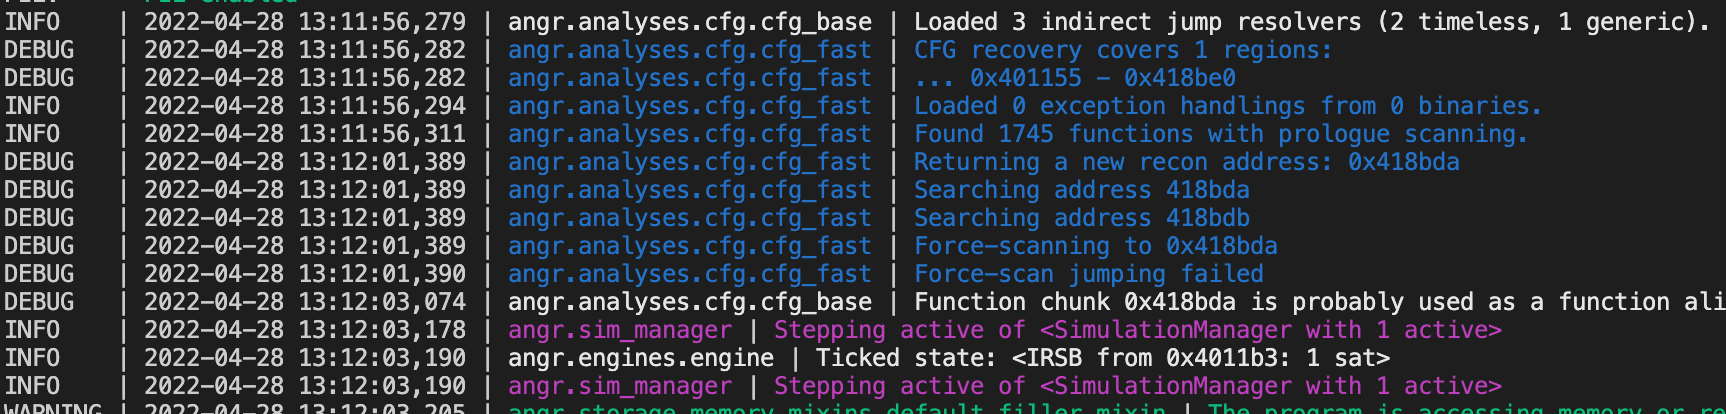
\includegraphics[width=\textwidth]{log-example}
    \end{center}
    \absfootnote{Check \codec{logging.root.manager.loggerDict} for existing loggers!}
    \absgraphic{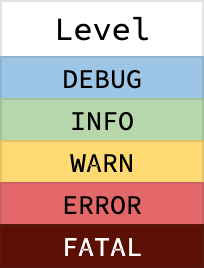
\includegraphics[width=2.5cm]{log-levels}}[9.2cm][-2cm]
    \absgraphic{
\includegraphics[width=0.5cm]{inside-out-anger}}[11.7cm][-4.75cm]
\end{frame}

\subsection{Debugging}
\begin{frame}{Debugging States}
    \begin{itemize}
        \item \codec{state.callstack}: addresses, flow.
        \item \codec{state.history}: data, constraints, jumps.
        \item \codec{state.inspect.b}: breakpoints!
    \end{itemize}
    \-\\
    \uncover<2->{Actually these aren't just for debugging!}
\end{frame}
\begin{frame}[fragile]{\code{state.callstack}}
    \begin{center}
        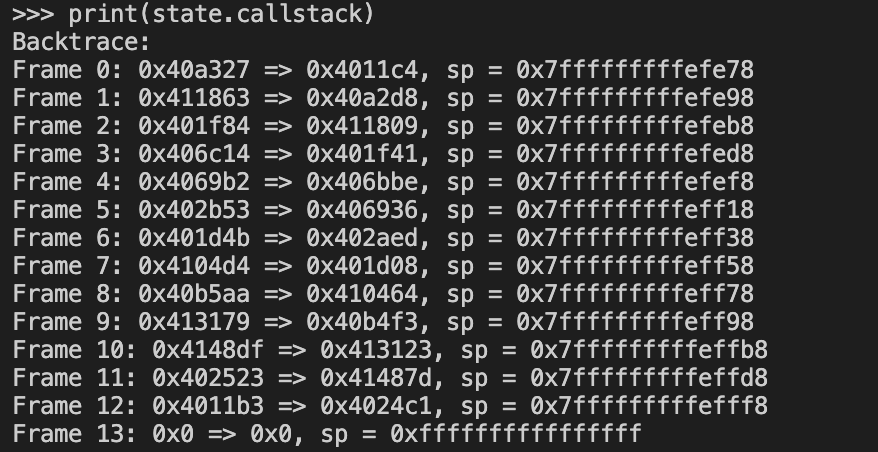
\includegraphics[height=3.5cm]{state-callstack}
    \end{center}
    \begin{block}<2->{Useful Stuff}
        \vskip-5pt
        \begin{lstlisting}[style=plainpy,gobble=12]
            print(state.callstack)    # Display backtrace.
            state.callstack.stack_ptr # Stack pointer (int).
            state.callstack.func_addr # Address of current function.
            state.callstack.ret_addr  # Return address.
        \end{lstlisting}
    \end{block}
    \morefootnote{https://docs.angr.io/core-concepts/states#the-callstack-plugin}
\end{frame}
\begin{frame}[fragile]{\code{state.history} -- Overview}\label{debugging-states}
    A collection of different iterables...
    \begin{itemize}
        \item<1-> \codec{.actions}: tracks data and constraints.
        \item<2-> \codec{.bbl\_addrs}: blocks executed to reach this state.
        \item<2-> \codec{.descriptions}: logs as strings.
        \item<2-> \codec{.jump\_guards}: branch constraints.
              \vskip5pt
        \item<2-> \codec{.events}: similar to \codec{.actions} but moar.
              \begin{itemize}
                  \item Useful for checking why states deadended.
              \end{itemize}
    \end{itemize}
    \morefootnote{https://docs.angr.io/core-concepts/states#the-history-plugin}
\end{frame}
\begin{frame}[fragile]{\code{state.history} -- Viewing}
    \begin{block}{Useful Stuff}
        \begin{itemize}
            \item {\footnotesize\codec{state.history.actions.hardcopy}}
                  \begin{itemize}
                      \item Turn the actions iterable into a list.
                  \end{itemize}
            \item {\footnotesize\codec{print(*state.history.actions, sep=`\textbackslash n')}}
                  \begin{itemize}
                      \item Prints each action on its own line.
                  \end{itemize}
        \end{itemize}
    \end{block}
\end{frame}
\begin{frame}[fragile,t]{\code{state.history.actions}}
    Tracks data (register/memory read and writes) and constraints.
    \vspace{-10pt}
    \begin{center}
        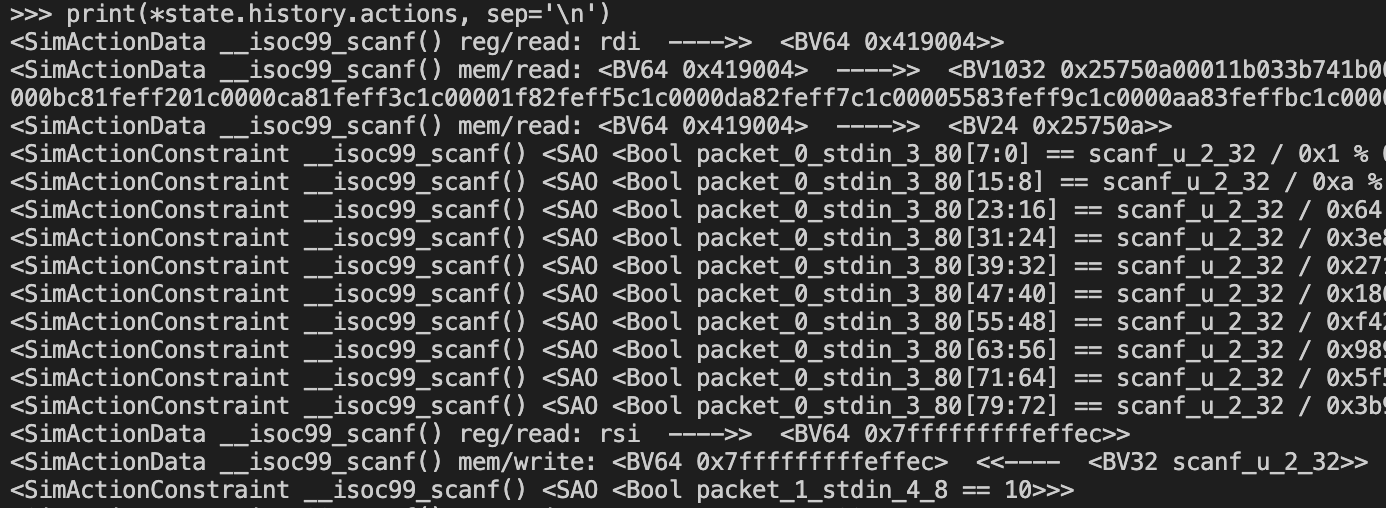
\includegraphics[height=4cm]{state-history-actions}
    \end{center}
    \begin{block}<2->{Useful Stuff}
        \vskip-5pt
        \begin{lstlisting}[style=plainpy,gobble=12]
            state.options |= sim_options.refs   # Track EVERYTHING!
        \end{lstlisting}
    \end{block}
    \begin{overlaytextblock}
        \begin{onlyenv}<2->
            \begin{textblock}{3}(4.3, -1.2)
                \begin{rotate}{-5}
                    \tiny
                    \parbox{26mm}{Add this before \\ constructing the simgr!}
                \end{rotate}
            \end{textblock}
        \end{onlyenv}
    \end{overlaytextblock}
\end{frame}
\begin{frame}[fragile]{\code{state.inspect.b\small(event\_type, **kwargs)}}
    \footnotesize
    \begin{block}{\code{event\_type}}
        \begin{itemize}
            \item \codec{mem\_read}, \codec{mem\_write}: memory is being read/written.
            \item \codec{reg\_read}, \codec{reg\_write}: register is being read/written.
            \item \codec{constraints}: new constraints are being added.
            \item \codec{call}: a \codec{call} instruction is hit.
            \item \codec{ret}: a \codec{ret} instruction is hit.
            \item \codec{symbolic\_variable}: a new symbolic variable is being created.
            \item \codec{syscall}: a syscall is being executed.
        \end{itemize}
    \end{block}
    \morefootnote{https://docs.angr.io/core-concepts/simulation#breakpoints}
\end{frame}
\begin{frame}[fragile]{\code{state.inspect.b\small(event\_type, **kwargs)}}
    \footnotesize
    \begin{block}{\code{when=}}
        \begin{itemize}
            \item \codec{BP\_BEFORE}: trigger before the breakpoint.
            \item \codec{BP\_AFTER}: trigger after the breakpoint.
        \end{itemize}
    \end{block}
    \begin{block}{\code{action=}}
        \begin{itemize}
            \item \codec{func}: execute your own Python handler.
            \item \codec{BP\_IPDB}: enter an IPython debugger.
            \item \codec{BP\_IPYTHON}: enter an IPython shell.
        \end{itemize}
    \end{block}
    \begin{block}{\code{**kwargs}}
        \begin{itemize}
            \item Different kwargs are available for each \codec{event\_type}! Check the link below.
        \end{itemize}
    \end{block}
    \morefootnote{https://docs.angr.io/core-concepts/simulation#breakpoints}
\end{frame}


\appendix
\section{\appendixname}
\frame{\tableofcontents}
\subsection{Tips}
\begin{frame}[fragile]{angr Tips}\label{tips}
    \begin{itemize}
        \item Breathe and relax.
        \item Always use angr in a virtual environment (e.g. \exref{https://docs.python.org/3/library/venv.html}{venv}, \exref{https://docs.conda.io/projects/conda/en/latest/user-guide/install/index.html}{conda}).
        \item Use a Jupyter notebook/IPython, or run scripts interactively \\(\codec{python3 -i script.py}) to easily play around with variables and methods.
        \item \codec{import monkeyhex} to conveniently view numbers as hex.
        \item Tab completion is your friend.
        \item The most updated documentation is the code itself.
    \end{itemize}
    \absgraphic{
\includegraphics[width=2cm, clip, trim=1cm 0 0 0]{kalm}}[5cm][-1.4cm]
\end{frame}
\subsection{angr Model}
\begin{frame}{angr Model (Link Galore)}
    \angrModelShowFlow{-1}
\end{frame}
\subsection{More Links}
\begin{frame}{More Links}
    \footnotesize
    \begin{itemize}
        \item Repo: \url{https://github.com/angr/angr}
        \item Docs (Book-like): \url{https://docs.angr.io/}
        \item API: \url{https://api.angr.io/}
        \item Examples: \url{https://docs.angr.io/examples}
        \item More Examples: \url{https://github.com/angr/angr-doc/blob/master/docs/more-examples.md}
        \item Attack Plan (Strategies): \url{https://github.com/bordig-f/angr-strategies}
        \item CFG (Wikipedia): \url{https://en.wikipedia.org/wiki/Control-flow_graph}
        \item CFG (1970s paper, a potentially interesting read, mathy/theoretical):
              \url{https://dl.acm.org/doi/10.1145/390013.808479}
    \end{itemize}
\end{frame}

\subsection{}
\begin{frame}{Questions?}
    \centering
    \includegraphics[width=0.8\textwidth]{questions-4}
\end{frame}

\end{document}
